\documentclass{report}

\input{../../Analisi/LatexTemp/preamble}
\input{../../Analisi/LatexTemp/macros}
\input{../../Analisi/LatexTemp/letterfonts}

\setlength{\parindent}{0pt}

\title{\Huge{Algebra e Geometria}\\Appunti}
\author{\huge{Alex Bastianini}}
\date{}
\pagenumbering{gobble}

\begin{document}

\maketitle
\newpage% or \cleardoublepage
% \pdfbookmark[<level>]{<title>}{<dest>}
\pdfbookmark[section]{\contentsname}{toc}
\tableofcontents
\pagebreak

\chapter{Sistemi lineari}
\section{Equazione lineare}
\dfn{Equazione lineare}{
Un' \textbf{equazione lineare} in n incognite e' un'equazione di tipo:
\[
  a_1x_1 + a_2x_2 + ... + a_nx_n = b
\]
dove $a_1,...,a_n,b \in \mathbb{R}$ sono i coefficenti e $x_1,...,x_n$ sono le incognite (tutte di primo grado).\\
Una \textbf{soluzione} e' una n-upla ordinata ($c_1,...,c_n$) che sostituita alle incognite rende vera l'equazione.
}
\section{Sistema lineare}
\dfn{Sistema lineare}{
  Un sistema lineare e' un insieme di equazioni lineari che devono valere contemporaneamente.
  \[
  \begin{cases}
  a_{11}x_1 + a_{12}x_2 + ... + a_{1n}x_n = b_1\\
  a_{21}x_1 + a_{22}x_2 + ... + a_{2n}x_n = b_2\\
  \vdots\\
  a_{m1}x_2 + a_{m2}x_2 + ... + a_{mn}x_n= b_3
  \end{cases}
\]
  Si chiama soluzione del sistema ogni n-upla $(c_1,...,c_n)$ che e' soluzione di ogni equazione del sistema. Un sistema e' \textbf{compatibile} se ammette almeno una soluzione.\\
  Il sistema si dice \textbf{omogeneo} se $\forall i \in [1,n] \to b_i = 0$, in questo caso esiste per forza la soluzione x = (0, 0,...,0).
}

\chapter{Matrici} 
\dfn{Matrice}{
  Una \textbf{matrice} A con m righe e n colonne e' una tabella (di numeri reali) dove $a_{ij}$ e' il coefficente di posto (i,j) della matrice A.
  \[
  A_{3\times4} = 
  \begin{pmatrix}
  a_{11} & a_{12} & a_{13} & a_{14}\\
  a_{21} & a_{22} & a_{23} & a_{24}\\
  a_{31} & a_{32} & a_{33} & a_{34}\\
  \end{pmatrix}
  \]
  
  L'insieme delle matrici di m righe e n colonne si indica con $M_{m\times n}(\mathbb{R})$. Una matrice e' \textbf{quadrata} quando m = n. La \textbf{trasposta} di una matrice A $A^T \in M_{n \times m}(\mathbb{R})$ e' la matrice che si ottiene scambiando le righe con le colonne ($a^T_{ij} = a_{ji}$).
}

Due matrici A e B sono uguali sse $\forall i,j. a_{ij} = b_{ij}$.\\
Una riga di una matrice $A_{m\times n}$ puo' essere vista come una matrice $1 \times n$, mentre una colonna puo' essere vista come una matrice $m\times 1$.
\section{Prodotti}
\dfn{Prodotto riga-colonna}{
  Date una riga $1\times n$ e una colonna $n \times 1$ aventi la stesssa lungezza, il loro prodotto e':
  \[
    \begin{pmatrix}
    a_1 & a_2 & \dots & a_n\\
    \end{pmatrix} \cdot \begin{pmatrix}
    b_1\\
    b_2\\
    \vdots\\
    b_n\\
    \end{pmatrix} = a_1b_1 + a_2b_2 + ... + a_nb_n \in \mathbb{R}
  \]
}
\dfn{Prodotto di due matrici}{
  Date due matrici $A\in M_{m\times k}$ e $B \in M_{k\times n}$, il loro prodotto e' una matrice $C\in M_{m\times n}$:
    \[
    A \cdot B = \begin{pmatrix}
    a_{11} & a_{12}\\
     \vdots \\
    a_{m1} & a_{m2}\\
    \end{pmatrix} \cdot \begin{pmatrix}
    b_{11} & ... & b_{1n}\\
    b_{12} & ... & b_{2n}\\
    \end{pmatrix} = \begin{pmatrix}
    c_{11} & ... & c_{1n}\\
    \vdots\\
    c_{m1} & ... & c_{mn} \\
    \end{pmatrix} = C\in M_{m\times n}
    \]
  Ogni elemento di C e' definito come segue:
  \[
    c_{ij} = (\text{riga i di A}) \cdot (\text{colonna j di B})
  \]
  Il prodotto BA non e' definito se non sono matrici quadrate, quindi \textbf{il prodotto non e' commutativo}.
}
\ex{Prodotto fra matrici}{
  \begin{enumerate}
    \item 
      \[
      \begin{pmatrix}
      1 & 3\\
      -4 & 5\\
      2 & -1\\
      0 & 2\\
      \end{pmatrix} \cdot \begin{pmatrix}
      1 & 0 & 2\\
      -1 & 1 & 0\\
      \end{pmatrix} = \begin{pmatrix}
      -2 & 3 & 2\\
      -9 & 5 & -8\\
      3 & -1 & 4\\
      -2 & 2 & 0\\
      \end{pmatrix}
      \]
    \item 
      \[
      \begin{pmatrix}
      1 & 0 & 2\\
      -1 & 1 & 0\\
      \end{pmatrix} \cdot \begin{pmatrix}
      1 & 3\\
      -4 & 5\\
      2 & -1\\
      0 & 2\\
      \end{pmatrix} = \text{undefined} 
      \]
      
  \end{enumerate}
}
\section{Somma}
\dfn{Somma}{
  Possiamo sommare due matrici A e B solo se hanno la stessa forma ($A,B\in M_{m\times n}$).
\[
  A+B=C \iff \forall c_{ij} = a{ij} + b{ij}
\]
}
\ex{Somma di matrici}{
  \begin{enumerate}
  \item 
    \[
    \begin{pmatrix}
    1 & 2\\
    3 & 4\\
    5 & 6\\
    \end{pmatrix} + \begin{pmatrix}
    2 & 4\\
    1 & 3\\
    6 & 5\\
    \end{pmatrix} = \begin{pmatrix}
    3 & 6\\
    4 & 7\\
    11 & 11\\
    \end{pmatrix}
    \]
   \item 
     \[
     \begin{pmatrix}
     1 & 2\\
     3 & 4\\
     5 & 6\\
     \end{pmatrix} + \begin{pmatrix}
     1 & 2\\
     3 & 4\\
     \end{pmatrix} = \text{undefined}
     \]

  \end{enumerate}
}
\section{Proprieta'}
\begin{itemize}
  \item (A+B)C = AC+BC (distributiva)
  \item C(A+B) = CA+CB
  \item $(AB)^T=B^TA^T$
  \item (AB)C = A(BC)
\end{itemize}

\section{Soluzioni di sistemi lineari}
E' possibile rappresentare un sistema lineare usando il prodotto di due matrici:
\[
  \begin{cases}
    a_{11}x_1 + a_{12}x_2 + ... + a_{1n}x_n = b_1\\
    a_{21}x_1 + a_{22}x_2 + ... + a_{2n}x_n = b_2\\
    \vdots\\
    a_{m1}x_2 + a_{m2}x_2 + ... + a_{mn}x_n= b_3
  \end{cases} \leftrightarrow \begin{pmatrix}
  a_{11} & a_{12} & ... & a_{1n}\\
  a_{21} & a_{22} & ... & a_{2n}\\
  \vdots\\
  a_{m1} & a_{m2} & ... & a_{mn}\\
  \end{pmatrix} \cdot 
  \begin{pmatrix}
  x_1\\
  x_2\\
  \vdots\\
  x_m\\
  \end{pmatrix} = 
  \begin{pmatrix}
  b_1\\
  b_2\\
  \vdots \\
  b_m \\
  \end{pmatrix} \to A\underline{x}=\underline{b}
\]
La matrice A si dice \textbf{incompleta}, mentre con $A|b$ si indica la matrice \textbf{completa}.
\[
A|b = 
\begin{pmatrix}
a_{11} & a_{12} & ... & a_{1n} & b_1\\
a_{21} & a_{22} & ... & a_{2n} & b_2\\
 \vdots\\
a_{m1} & a_{m2} & ... & a_{mn} & b_m\\
\end{pmatrix}
\]
Una matrice si dice a \textbf{scala} se:
\begin{itemize}
  \item Le righe vuote (dove tutti gli elementi sono 0) si trovano in fondo.
  \item Il primo elemento diverso da 0 di ogni riga (detto \textbf{pivot}) si trova piu' a destra della riga sovrastante.
\end{itemize}

\ex{Matrici a scala}{\label{scala}
  \begin{enumerate}
    \item La seguente matrice e' a scala (i pivot sono sottolineati):
    \[
    \begin{pmatrix}
    \underline{1} & 3 & 5 & 6\\
    0 & \underline{2} & 3 & 4\\
    0 & 0 & \underline{3} & 2\\
    0 & 0 & 0 & 0\\
    \end{pmatrix}
    \]
    
  \end{enumerate}
}

Data una matrice A a scala, si chiama \textbf{rango righe} di A (rr(A)) il numero di righe non nulle di A. Nell'esempio \ref{scala} il rango righe della matrice e' 3.\\ \\
Sia $A\underline{x} = \underline{b}$ un sistema lineare a scala con incognite $x_1, ..., x_n$:
\begin{itemize}
  \item il sistema ha soluzioni $\iff$ $rr(A) = rr(A|b)$
  \item se $rr(A)=rr(A|b)=n \implies$ esiste una sola soluzione
  \item se $rr(A)=rr(A|b)=k,k < n \implies$ esistono infinite soluzioni che dipendono da n-k parametri (controllare!)
\end{itemize}
\ex{Numero di soluzioni}{
  \begin{enumerate}
  \item  \[
A|b = \begin{pmatrix}
1 & 0 & 5\\
0 & 0 & 1\\
\end{pmatrix}
\]
      $rr(A)=1\neq rr(A|b)=2$, quindi non ci sono soluzioni.
    \item    
          \[
A|b = \begin{pmatrix}
1 & 0 & 5\\
0 & 1 & 1\\
\end{pmatrix}
\]
      $rr(A)=rr(A|b)=2=n$, quindi esiste una sola soluzione.
      \item 
        \[      
A|b = \begin{pmatrix}
1 & 2 & 5\\
\end{pmatrix}
        \]
        $rr(A)=rr(A|b)=1<n=2$, quindi esistono infinite soluzioni dipendenti da 2-1=1 variabili.
  \end{enumerate}
}
\section{Gauss}
\dfn{Equivalenza fra sistemi lineari}{
  Due sistemi lineari si dicono \textbf{equivalenti} se hanno le stesse soluzioni.
}
Per risolvere un sistema lineare A\underline{x}=\underline{b}, lo trasformiamo in un sistema \textbf{equivalente} A'x=b' tale che A'x=b' sia a scala.\\
Le seguenti operazioni trasformano un sistema ad uno ad esso equivalente:
\begin{itemize}
\item Scambio di due equazioni.
  \item Moltiplicazione di una equazione per un numero reale $c\in\mathbb{R}$, con $c\neq0$.
    \item Sostituzione della equazione j-esima con la somma della equazione j-esima piu' l'equazione i-esima moltiplicata per $a\in\mathbb{R}$.
\end{itemize}
A queste operazioni corrispondono delle \textbf{operazioni elementari} sulle righe (lavorando quindi sulle matrici):
\dfn{Operazioni elementari}{
  Sono le seguenti operazioni fra le righe di una matrice:
  \begin{itemize}
  \item Scambio di due righe $R_i \leftrightarrow R_j$.
    \item Moltiplicazione di una righa per $c\in\mathbb{R}, c\neq0$ $R_i \to cR_i$.
      \item $R_j \to R_j + aR_i, a\in\mathbb{R}$.
  \end{itemize}
}
Tramite l'algoritmo di Gauss, possiamo trasformare una matrice in una matrice a scala per righe.
\dfn{Algoritmo di Gauss}{
  Guardare su virtuale...
}
\nt{
  La matrice a scala non e' univocamente determinata.
}
\chapter{Spazi vettoriali}
\section{Introduzione}
\dfn{Spazio vettoriale}{
  Uno spazio vettoriale su un \textbf{campo} F (per noi sempre $ \mathbb{R} $) e' una struttura algebrica ($ V,F,+,\cdot $) dove V e' un insieme per cui e' definita una somma ($ \forall v,u \in V. \exists s \in V. s=v+u $) e un prodotto per numeri \textbf{scalari} ($ \forall v \in V,\forall \lambda \in F. \exists u \in V.u=\lambda\cdot v $) dove valgono le seguenti proprieta':
\begin{enumerate}
\item Somma
  \begin{itemize}
  \item Commutativa
    \item Associativa
    \item Esistenza elemento \textbf{neutro}: $ \exists \underline{0} \in V. \forall v \in V. v+\underline{0} = v $
    \item Esistenza elemento \textbf{opposto}: $ \forall v \in V. \exists -v \in V. v+(-v)=\underline{0} $
  \end{itemize}
    Si nota che per tali proprieta' (V,+) forma un \textbf{gruppo abeliano}.
\item Prodotto 
  \begin{itemize}
    \item Distributiva a destra: $ \forall v,u \in V,\forall \lambda \in F. \lambda(v+u)=\lambda v + \lambda u   $
    \item Distributiva a sinistra: $ \forall v \in V,\forall \lambda,\mu \in F.(\lambda + \mu)v=\lambda v + \mu v $
    \item Associativa: $ \forall v \in V,\forall \lambda,\mu \in F.(\lambda\mu)v = \lambda(\mu v) $
  \item Esistenza elemento \textbf{neutro}: $ \exists 1 \in F.\forall v \in V. 1\cdot v = v $ 
  \end{itemize}
\end{enumerate}     
}
Dalla definizione di spazio vettoriale seguono altre proprieta' interessanti:
\begin{itemize}
\item Il vettore nullo $ \underline{0} $ e' \textbf{unico}
\item Per ogni vettore $ v $ il suo opposto $ -v $ e' \textbf{unico}
\item L'elemento neutro della somma del campo F ha la proprieta' \textbf{assorbitiva} rispetto al prodotto scalare: $ \forall v \in V.0v=\underline{0} $
\item Legge di cancellazione del prodotto: $ \forall v \in V,\forall \lambda \in F.\lambda v = 0 \iff v = \underline{0} \lor \lambda = 0 $
\item $ \forall v \in V,\forall \lambda \in F.(-\lambda)v = \lambda(-v) = -\lambda v$
\end{itemize}
\nt{
  Un insieme contenente solo il vettore nullo e' uno spazio vettoriale, e viene chiamato \textbf{banale}:
  \[
  V=\{\underline{0}\} \implies \text{Spazio vettoriale banale}
  \]
}
\ex{Spazio vettoriale}{
  Dimostriamo che $ (\mathbb{R}^2,\mathbb{R},+,\cdot) $ e' uno spazio vettoriale, dove $ \mathbb{R}^2 = \{(x,y)|x,y\in\mathbb{R}\} $:
  \begin{itemize}
  \item Si puo' dimostrare che valgono la prop. comm. e ass. della somma
  \item Si puo' dimostrare che valgono la prop. ass. e distr. del prodotto scalare
  \item L'elemento neutro della somma e' il vettore $ v=(0,0) $, e ogni vettore (x,y) ha il suo opposto (-x,-y)
  \item L'elemento neutro del prodotto e' lo scalare 1
  \end{itemize}
  Si nota che esiste una corrispondenza biunivoca fra i vettori di $ \mathbb{R}^2 $ e i punti del piano cartesiano, quindi ogni vettore puo' essere rappresentato come una "freccia" che parte dall'origine (il vettore nullo) e arriva al punto cartesiano corrispondente:\\
  \begin{align*}
 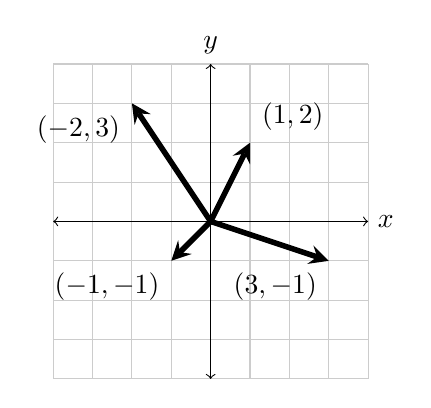
\begin{tikzpicture}[scale=0.5]
  \draw[thin,gray!40] (-4,-4) grid (4,4);
  \draw[<->] (-4,0)--(4,0) node[right]{$x$};
  \draw[<->] (0,-4)--(0,4) node[above]{$y$};
  \draw[line width=2pt,-stealth](0,0)--(1,2) node[anchor=south west]{$(1, 2)$};
  \draw[line width=2pt,-stealth](0,0)--(-2,3) node[anchor=north east]{$(-2, 3)$};
  \draw[line width=2pt,-stealth](0,0)--(3,-1) node[anchor=north east]{$(3, -1)$};
  \draw[line width=2pt,-stealth](0,0)--(-1,-1) node[anchor=north east]{$(-1, -1)$};
\end{tikzpicture}
  \end{align*}
  Esempio di somma di due vettori $ v=(1,2) $ e $ u=(3,-1) $:
  \begin{align*}
    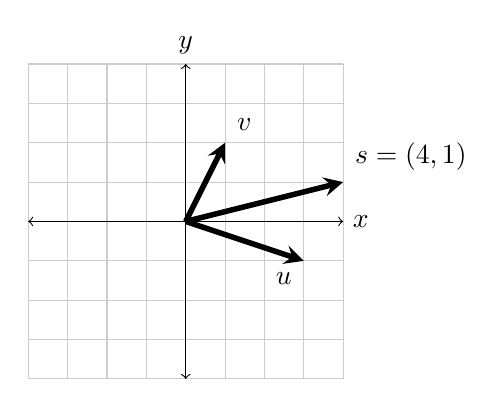
\begin{tikzpicture}[scale=0.5]
      \draw[thin,gray!40] (-4,-4) grid (4,4);
      \draw[<->] (-4,0)--(4,0) node[right]{$x$};
      \draw[<->] (0,-4)--(0,4) node[above]{$y$};
      \draw[line width=2pt,-stealth](0,0)--(1,2) node[anchor=south west]{$v$};
      \draw[line width=2pt,-stealth](0,0)--(3,-1) node[anchor=north east]{$u$};
      \draw[line width=2pt,-stealth](0,0)--(4,1) node[anchor=south west]{$s=(4, 1)$};
    \end{tikzpicture}
  \end{align*}
  Esempio di prodotto scalare $ \lambda v $, dove $ \lambda = -\frac{1}{3}, v = (3,1) $:
  \begin{align*}
    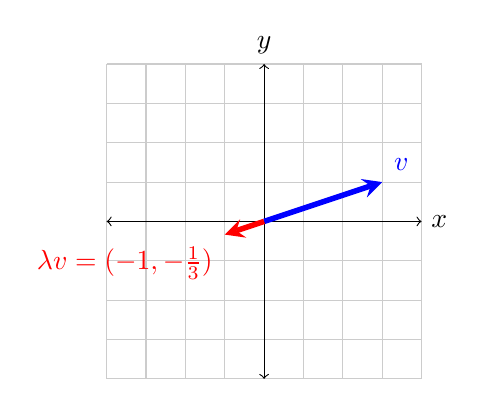
\begin{tikzpicture}[scale=0.5]
      \draw[thin,gray!40] (-4,-4) grid (4,4);
      \draw[<->] (-4,0)--(4,0) node[right]{$x$};
      \draw[<->] (0,-4)--(0,4) node[above]{$y$};
      \draw[line width=2pt,blue,-stealth](0,0)--(3,1) node[anchor=south west]{$v$};
      \draw[line width=2pt,red,-stealth](0,0)--(-1,-1/3) node[anchor=north east]{$\lambda v = (-1,-\frac{1}{3})$};
    \end{tikzpicture}
  \end{align*}
}
\section{Sottospazi}
\dfn{Sottospazio}{
  V sp. vett., $ U \subseteq V $ di dice \textbf{sottospazio} se:
  \begin{enumerate}
  \item $ U \neq \emptyset $
  \item $ \forall a,b \in U. a+b \in U $(chiusura rispetto alla somma)
  \item $ \forall \lambda, v \in U. \lambda v \in U $(chiusura rispetto al prodotto per scalari)
  \end{enumerate}
}

\nt{
  Sia $ U\leq V $ (U sottospazio V), per la proprieta' 3 si ha che ogni sottospazio contiene il vettore nullo $ \underline{0} $, perche' $ \forall v \in U.0v=\underline{0} $, quindi:
  \begin{enumerate}
    \item O $ U = \{\underline{0}\} $ (sottospazio banale),
    \item oppure $ U\neq \{\underline{0}\} $, allora $ \exists u \in V \neq \underline{0} $, ed esistono anche tutti i \textbf{multipli} di u (che sono infiniti). 
  \end{enumerate}
  (Da notare la somiglianza con i sistemi lineari: se ci sono "soluzioni" o ce ne' una, o ce ne sono infinite)
}

\subsection{Sottospazi di $ \mathbb{R}^2 $}
Lo spazio vettoriale $ \mathbb{R}^2 $ e' in corrispondenza diretta con i punti del piano cartesiano.\\
Sia $ U \leq \mathbb{R}^2 $, si ha che:
\begin{itemize}
  \item $ U=\{(0,0)\} $, oppure
  \item $ \exists u \in U. u \neq \underline{0} $, e di conseguenza tutti i suoi multipli, ovvero la \textbf{retta} $ r_u $ passante per l'origine.
    \item $ \exists v \in U $ con $ v \not\in r_u $, quindi esistono anche tutti i punti ottenuti sommando punti di $ r_u $ e $ r_v $ e le rette passanti per questi punti e l'origine, che si puo' dimostrare che occupano tutto il piano $ \mathbb{R}^2 $.
\end{itemize}

\ex{Possibili sottospazi di $ \mathbb{R}^2 $}{
  \begin{enumerate}
  \item $ U=\{\underline{0}\} $:
  \begin{align*}
    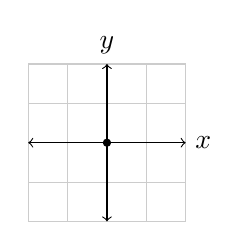
\begin{tikzpicture}[scale=0.5]
      \draw[thin,gray!40] (-2,-2) grid (2,2);
      \draw[<->] (-2,0)--(2,0) node[right]{$x$};
      \draw[<->] (0,-2)--(0,2) node[above]{$y$};
      \fill (0,0) circle[radius=3pt];
    \end{tikzpicture}
  \end{align*}

\item $ U=\{(0,0),(1,2),(2,4),(-1,-2),...\} $, ovvero $ U=\{(\lambda 1,\lambda 2)|\lambda \in \mathbb{R}\}=r_v $:
  \begin{align*}
    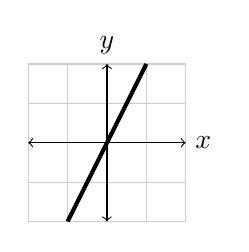
\begin{tikzpicture}[scale=0.5]
      \draw[thin,gray!40] (-2,-2) grid (2,2);
      \draw[<->] (-2,0)--(2,0) node[right]{$x$};
      \draw[<->] (0,-2)--(0,2) node[above]{$y$};
      \draw[line width=1.5pt,domain=-1:1] plot (\x, \x*2);
    \end{tikzpicture}
  \end{align*}
\item Se aggiungiamo il vettore $ u=(1,1) \not\in r_v $ a $ U $, $ U=\{(x,y)|x,y\in\mathbb{R}\}=\mathbb{R}^2 $:
  \begin{align*}
    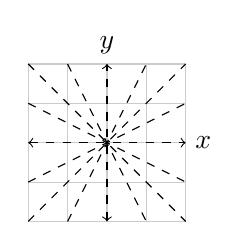
\begin{tikzpicture}[scale=0.5]
      \draw[thin,gray!40] (-2,-2) grid (2,2);
      \draw[dashed,<->] (-2,0)--(2,0) node[right] {$x$};
      \draw[dashed,<->] (0,-2)--(0,2) node[above] {$y$};
      \draw[dashed,domain=-1:1] plot (\x, \x*2);
      \draw[dashed,domain=-2:2] plot (\x, \x);
      \draw[dashed,domain=-2:2] plot (\x, \x/2);
      \draw[dashed,domain=-1:1] plot (\x, {\x*(-2)});
      \draw[dashed,domain=-2:2] plot (\x, {\x*(-1)});
      \draw[dashed,domain=-2:2] plot (\x, {\x*(-1/2)});
    \end{tikzpicture}
  \end{align*}
  \end{enumerate}
}

\section{Combinazioni lineari e generatori}
\dfn{Combinazione lineare}{
  V SV con $ v_1,...,v_n \in V $. $ v \in V $ si dice \textbf{combinazione lineare} di $ v_1,...,v_n $ se esistono $ \lambda_1,...,\lambda_n \in \mathbb{R} $ tali che $ v = \lambda_1v_1+...+\lambda_nv_n $. Quindi:
  \[
    v\in<v_1,...,v_n> = \{\lambda_1 v_1+...+\lambda_nv_n|\lambda_1,...,\lambda_n \in \mathbb{R}\}\text{ (Insieme di combinazioni lineari di $ v_1,...,v_n $)}
  \]
}
\mprop{}{ \label{siSV}
  Sia V SV e $ \{v_1,...,v_n\} \in V $, allora:
  \[ <v_1,...,v_n> \leq V \]
  Inoltre, se $ Z \leq V \land v_1,...,v_n \in Z $, allora:
  \[ <v_1,...,v_n> \leq Z \] 
}
Cio' significa che l'insieme di combinazioni di \textbf{qualunque} sotto-insieme di vettori di uno spazio vettoriale e' uno sotto-spazio vettoriale. Inoltre tale sotto-spazio e' il piu' piccolo contenente i vettori del sotto-insieme.
\dfn{Generatore}{
  Dati V SV e $ v_1,...,v_n \in V $, si dice che $ v_1,...,v_n $ \textbf{generano} V se $ V = <v_1,...,v_n> $ 
}
\ex{Generatore $ \mathbb{R}^3 $}{
  $ \{(1,0,0),(0,1,0),(0,0,1)\} $ generano $ \mathbb{R}^3 $, cioe' $ \mathbb{R}^3 = \{\lambda_1e_1+\lambda_2e_2+\lambda_3e_3|\lambda_1,\lambda_2,\lambda_3 \in \mathbb{R}\} $ che ovviamente si puo' fare.
}

\mprop{}{ \label{comb}
  Dati V SV e $ v_1,...,v_n, v \in V $:
  \[
    v\text{ e'  \textit{combinazione lineare} di } v_1,...,v_n \iff <v_1,...,v_n> = <v_1,...,v_n,v>
  \]
}
\section{Vettori linearmente indipendenti}
\dfn{}{
  Dati V SV e $ v_1,...v_n \in V $, $ v_1,...,v_n $ si dicono \textbf{linearmente indipendenti} sse l'\textbf{unica} loro combinazione lineare che da il vettore nullo e' quella con scalari tutti uguali a 0, cioe' se vale:
  \[
  \lambda_1v_1+...+\lambda_nv_n = 0 \implies \lambda_1,...,\lambda_n = 0
  \]
}
\mprop{}{
  Se S e' un insieme di vettori linearmente indipendenti, ogni suo sotto-insieme e' ancora linearmente indipendente. (L'insieme vuoto e' linearmente indipendente)
}
\mprop{}{ \label{dip}
  Dati V SP e $ v_1,...,v_n \in V $, $ v_1,...,v_n $ sono \textbf{linearmente dipendenti} sse uno di essi e' combinazione lineare degli altri. 
}
\pf{Dimostrazione}{
  Dimostro entrambe le direzioni:
  \begin{itemize}
  \item $ \Rightarrow $ Sapendo che $ v_1,...,v_n $ sono linearmente dipendenti (H1), devo dimostrare che $ \exists r \in [1,n].v_r \in <v_1,...,v_n>\setminus v_r $. Da H1, sappiamo che $ \exists \lambda_r \neq 0.\lambda_1v_1+...+\lambda_nv_n=0 $, quindi $ v_r = -\frac{1}{\lambda_r}(\lambda_1v_1+...+\lambda_nv_n) $. Allora $ v_r $ e' combinazione lineare degli altri.
\item $ \Leftarrow $ Sapendo che $ v_r \in <v_1,...,v_n>\setminus v_r $ (H1), devo dimostrare che $ v_1,...,v_n $ sono linearemente dipendenti. Per H1 $ v_r = \lambda_1v_1+...+\lambda_nv_n $, quindi $ \lambda_1v_1+...+\lambda_nv_n+(-1)v_r = 0 $. Cio' dimostra che una combinazione lineare di $ v_1,...v_n $ e' risultata 0 quando uno dei fattori scalari era diverso da 0 (-1), quindi $ v_1,...v_n $ sono linearmente dipendenti.
  \end{itemize}
}
\cor{}{
  \textbf{Due} vettori sono lin dip $ \iff $ unodi essi e' multiplo dell'altro
}
\ex{}{
  $ (a,b,c) $ e $ (d,e,f) $ sono linearmente dipendenti solo se (con $ \lambda, \mu \neq 0 $):
  \begin{itemize}
    \item $ (a,b,c) = \lambda(d,e,f) = (\lambda d, \lambda e, \lambda f) $
    \item $ (d,e,f) = \mu(a,b,c) = (\mu a, \mu b, \mu c) $
  \end{itemize}
  Ma se vale il primo allora $ \mu = \frac{1}{\lambda}  $, quindi i due vettori sono multipli. 
}
\mprop{}{
  L'insieme di soluzioni di un sistema lineare omogeneo e' sempre uno sottospazio.
}
\ex{}{
  $ \begin{pmatrix}
  0 & 3 & 0\\
  7 & 9 & 0\\
  0 & 0 & 0\\
  1 & 1 & 0\\
  \end{pmatrix} $ ha sempre almeno una soluzione (il vettore nullo $ \underline{0} $).
}
\mprop{}{ \label{exGLI}
  Sia $ V = <v_1,...,v_n> \neq \{\underline{0}\} $. Allora esiste un sottoinsieme di vettori linearmente indipendenti di $ \{v_1,...,v_n\} $ che genera V.
}
\pf{Dimostrazione}{
  Dimostriamo in modo algoritmico:
  \begin{enumerate}
  \item Se $ v_1,...,v_n $ sono lin. ind., allora la prop. e' dimostrata. 
  \item Altrimenti, per il teo. \ref{dip}, esiste un vettore $ v_r \in \{v_1,...,v_n\} $ tale che questo e' combinazione lineare degli altri. Rimuoviamo quindi tale vettore dai generatori, e per \ref{comb} $ <v_1,...,v_n> = <v_1,...,v_n>\setminus v_r = V $. Tornare quindi al passo 1.
  \end{enumerate}
  Dopo un numero finito di passi (fino al massimo ad avere solo un elemento), si arriva a un insieme di vettori dove nessuno e' combinazione lineare degli altri, quindi per \ref{dip} si ha un insieme di vettori lin. ind. che generano V. 
}
\dfn{Base}{
  Un insieme di vettori $ v_1,...,v_n $ si dice \textbf{base} di $ V $ se:
  \begin{enumerate}
    \item $ v_1,...,v_n $ generano $ V $, quindi $ V = <v_1,...,v_n> $
    \item $ v_1,...,v_n $ sono linearmente indipendenti
  \end{enumerate}
}
\ex{}{
  \begin{enumerate}
    \item $ \{(1,0),(0,1)\} $ e' base di $ \mathbb{R}^2 $:
      \begin{enumerate}
        \item vera (gia visto)
        \item sono le righe non nulle di una matrice a scala
      \end{enumerate}
    \item $ \{(1,0),(0,1),(1,2)\} $ non sono una base:
      \begin{enumerate}
      \item generano $ \mathbb{R}^2 $
      \item pero' non sono indipendenti ($ (1,2) $ e' comb. lin. degli altri)
      \end{enumerate}
    \item $ \{(1,2,0),(0,5,0)\} $:
      \begin{enumerate}
        \item sono linearmente indipendenti (non sono uno il multiplo dell'altro)
        \item ma non generano $ \mathbb{R}^3 $, perche' due vettori individuano solo un piano
      \end{enumerate}
  \end{enumerate}
}
\dfn{}{
  Un SV si dice finitamente generato se ha un insieme finito di generatori.\\
  Cioe' se esistono $ v_1,...,v_n \in V.V = <v_1,...,v_n>$.
}
\ex{}{
  \begin{enumerate}
    \item $ \mathbb{R}^n $ e' finitamente generato: $ \mathbb{R}^n = <(1,0,...,0),...,(0,...,0,1)> $ 
  \item $ \mathbb{R}[x] $ (polinomi) non e' finitamente generato (non c'e' un numero finito di polinomi che puo' generare ogni polinomio di ogni grado)
  \end{enumerate}
}
\mprop{}{
  Sia V SV f.g. (finitamente generato), allora V ha una base.\\
  Nota: se $ V = \{\underline{0}\} $, allora V ha base $ \emptyset $ (e non $ \{\underline{0}\} $ perche' la dimensione di V e' 0, quindi per convenzione anche la sua base deve avere 0 vettori).
}
\pf{Dimostrazione}{
  Sia $ V = <v_1,...,v_n> $, per \ref{exGLI} esiste un sottoinsieme di $ \{v_1,...,v_n\} $ linearmente indipendente che genera V, quindi per def. base esiste una base di V.
}
\nt{
  Una base si ottiene cancellando i generatori superflui (combinazioni lineari degli altri)
}
\dfn{Basi canoniche}{
  Sono le basi "belle" per ogni SV:
  \begin{enumerate}
    \item $ \mathbb{R}^n, B = \{(1,0,0,...,0),(0,1,0,...,0),...,(0,0,...,1)\} $
    \item $ \mathbb{R}_n[x] $ (polinomi di grado max. n), $ B = \{x^n,...,x,1\} $
    \item $ M_{m \times n} $
  \end{enumerate}   
}
\thm{Completamento}{
  Sia $ V $ SV f.g. e $ B = \{w_1,...,w_n\} $ base di $ V $. Siano $ \{v_1,...,v_m\} \in V$ lin. indip:
  \begin{itemize}
  \item $ m \leq n $
  \item possiamo aggiungere a $ v_1,...,v_m $ $ m-n $ vettori di $ B $ in modo da ottenere una base
  \end{itemize}
}
\cor{}{
  Se V f.g. allora due basi di V hanno lo stesso numero di elementi.
}
\pf{}{
  Siano $ B_1,B_2 $ basi di $ V $. $ B_1 = \{v_1,...,v_n\} $ e $ B_2 = \{w_1,...,w_k\} $. Prendiamo come base di V $ B = B_1 $ e vediamo $ B_2 $ semplicemente come un insieme di vettori lin. ind., quindi per il teo. di compl. abbiamo che $ k \leq n $. Ripetendo questo passaggio invertendo $ B_1 $ e $ B_2 $, otteniamo $ n \leq k $. Allora per soddisfare entrambe le ipotesi abbiamo che n = k.
}
\dfn{Dimensione dello SV}{
  La dimensione di uno spazio vettoriale e' il numero di vettori in una base.
}
\ex{}{
  \begin{itemize}
    \item $ dim\mathbb{R}^n = n$
    \item $ dim \mathbb{R}_n[x] = n+1$
    \item $ dim M_{m \times n} = m \times n$
  \end{itemize}
}
\dfn{Massimale e minimale}{
  Un insieme $ S $ si dice \textbf{massimale} (\textbf{minimale}) con la proprieta $ \mathcal{P} $ su $ S $ se $ S $ ha $ \mathcal{P} $ e ogni sovrainsieme (sottoinsieme) proprio di $ S $ non ha (piu') $ \mathcal{P} $.
}
Proprieta' equivalenti:
\begin{itemize}
\item $ \{v_1,...,v_n\} $ e' base $ \iff  $ e' un insieme minimale di generatori
\item $ \{v_1,...,v_n\} $ e' base $ \iff $ e' un insieme massimale di vettori linearmente indipendenti
\end{itemize}
\mprop{}{
Sia V SV e $ W \leq V $:
\begin{itemize}
\item $ dim W \leq dim V $
\item $ dim W = dim V \implies V = W $
\end{itemize}
}
\pf{}{
  \begin{enumerate}
    \item Sia $ \{w_1,...,w_k\} $ una base di $ W $, $ w_1,...,w_k $ sono k vettori di V lin. ind., quindi per il teo. compl $ k \leq dim V $.
  \item Se $ k = dim V $, per il teo. compl., aggiungedo a $ \{w_1,...,w_k\} \text{(lin. ind.)} 0$ vettori allora diventa base di $ V $. Allora e' gia base di $ V $.
  \end{enumerate}
}
\mprop{GEL (Generare equivale a indipendenza lineare)}{
  Sia V SV di dim n, allora sono equivalenti (se vale uno valgono tutti):
  \begin{enumerate}
  \item $ \{v_1,...,v_n\} $ e' base di V
  \item $ \{v_1,...,v_n\} $ sono lin. ind.
  \item $ \{v_1,...,v_n\} $ generano V
  \end{enumerate}
}
\pf{}{
  E' ovvio che $ 1 \implies 2 $ e $ 1 \implies 3 $.\\
  $ 2 \implies 1 $ Per teo. compl., dato che $ v_1,...,v_n $ sono lin. ind., posso aggiungere $ dim V - n = 0 $ vettori per ottenere una base, quindi sono gia una base.\\
  $ 3 \implies 2 $ Se $ v_1,...,v_n $ fossero dipendenti, potrei cancellarne qualcuno e ottenerne una base di meno di n elementi. Ma questo e' assurdo perche' tutte le basi di V hanno n elementi. Quindi sono lin. ind.
}
\ex{}{
  Per controllare che $ \{2x,5,x^2\} $ sono una base di $ R_2[x] $, basta dimostrare che siano lin. ind. (dato che $ 3 = dim R_2[x] $)
}
\mprop{}{
  Sia $ B = \{v_1,...,v_n\} $ base ordinata di V SV e $ v \in V $, allora esistono \textbf{unici} $ \lambda_1,...,\lambda_n \in \mathbb{R}$ tale che:
  \[
  v = \lambda_1v_1+...+\lambda_nv_n
\]
}
\pf{}{
  Dato che $ B $ e' un insieme di generatori (per def. base), si ha che per def. generatori $ \exists \lambda_1,...,\lambda_n $ tali che:
  \[v=\lambda_1v_1+...+\lambda_nv_n \] 
  Dimostriamo ora l'unicita' prendendo $ \mu_1,...,\mu_n $ per cui:
  \[v = \mu_1v_1+...+\mu_nv_n \]
  Sottraiamo a questa uguaglianza $ v $ a sinistra e $ \lambda_1v_1+...+\lambda_nv_n $ a destra (possiamo farlo perche' abbiamo dimostrato che sono uguali) e otteniamo:
  \[
    0 = (\mu_1-\lambda_1)v_1 + ... + (\mu_n-\lambda_n)v_n 
  \]
  Dato che $ v_1,...,v_n $ sono linearmente indipendenti, una loro combinazione lineare e' 0 sse $ (\mu_1 - \lambda_1) = ... = (\mu_n - \lambda_n) = 0 $. Quindi abbiamo che $ \mu_1 = \lambda_1,...,\mu_n = \lambda_n $, e quindi abbiamo dimostrato l'unicita.
}
\dfn{}{
  Gli scalari $ \lambda_1,...,\lambda_n \in \mathbb{R}. v = \lambda_1v_1+...+\lambda_nv_n $ si dicono le \textbf{coordinate} di V rispetto alla base $ \beta $, e si scrive:
  \[
    (v)_{\beta} = (\lambda_1,...,\lambda_n) 
  \]
}
\section{Algotirmo di Gauss Diretto}
Possibile grazie a due teoremi:
\thm{}{
  Le operazioni elementari sulle righe di una matrcie non cambiano il sottospazio generato dalle righe stesse.
}
\pf{Dimostrazione}{
  Mostriamo per ogni operazione elementare come non cambia il sottospazio generato dalle sue righe:
  \begin{itemize}
  \item $ R_i \leftrightarrow R_j $ ovvio
  \item $ R_i \leftrightarrow \lambda R_i $ ovvio
  \item $ R_i \leftrightarrow R_i + \lambda R_j $ vero per prop. \ref{siSV}
  \end{itemize}
}
\thm{}{
  Le righe non nulle di una matrice a scala sono linearmente indipendenti.
}
Ci permette di trovare una base del sottospazio generato da alcunni vettori di $ \mathbb{R}^n $
\ex{}{
  Sia $ W = <(1,1,3,0),(2,2,5,1),(1,1,4,-1)> \leq \mathbb{R}^4 $, trovare una base di W.
  \begin{itemize}
  \item Costruiamo una matrice che ha per righe i tre vettori:
    \[
    \begin{pmatrix}
    1 & 1 & 3 & 0\\
    2 & 2 & 5 & 1\\
    1 & 1 & 4 & -1\\
    \end{pmatrix}
    \]
  \item Usiamo l'algoritmo di Gauss per ridurre la matrice in scala:
    \[
    \begin{pmatrix}
    1 & 1 & 3 & 0\\
    0 & 0 & -1 & 1\\
    0 & 0 & 0 & 0\\
    \end{pmatrix}
    \]
  \item Dato che abbiamo usato solo operazioni lineari, per prop. a $ <(1,1,3,0), (0,0,-1,1)> = <(1,1,3,0),(2,2,5,1),(1,1,4,-1)> $. Inoltre, per prop. b sappiamo che i due vettori nuovi sono lin. ind., quindi $ <(1,1,3,0),(0,0,-1,1)> $ e' una base (quindi $ dim W = 2 $)
  \end{itemize}
}
\chapter{Applicazioni lineari}
\section{Cos'e' una applicazione lineare}
\dfn{Applicazione lineare}{
  Siano $ V,W $ SV, $ f:V\to W $ si dice \textbf{applicazione lineare} sse:
  \begin{itemize}
    \item $ f(v+w) = f(v) + f(w) $
    \item $ f(\lambda v)=\lambda f(v) $
    \item $ f(0_V) = 0_W $
  \end{itemize}
  Morfismo di gruppi addittivi
}
\ex{}{
  \begin{enumerate} 
  \item $ V = \{f:\mathbb{R}\to\mathbb{R} \text{derivabili}\}, W = \{f:\mathbb{R}\to\mathbb{R}\} $:
    \[
    D V\to W
    \]
    \[
    f\to Df=f'
    \]
    \begin{itemize}
    \item $ D(f_1+f_2) = Df_1 + Df_2 $ ok
    \item $ D(\lambda f) = \lambda D(f) $ ok
    \end{itemize}
  \item $ f:\mathbb{R}^2\to\mathbb{R}^3 $ $ (x_1,x_2)\to(x_1,2x_2,-x_1) $ e' lineare
  \item $ f:\mathbb{R}^3\to\mathbb{R}^2 $ $ (x_1,x_2,x_3)\to(3x_2,-x_1+x_3+1) $ non e' lineare (il +1 la trolla)
  \item $ A \in M_{m\times n}(\mathbb{R}) $ $ L_A: \mathbb{R}^n\to\mathbb{R}^m $ $ \underline{x}=(x_1,...,x_n)\to A \underline{x} (m \times n \cdot n \times 1)$ e' lineare
  \end{enumerate}
}
\section{Nucleo e immagine}
\dfn{}{
  Siano $ A,B $ insiemi. $ f:A\to B $. $ Imm f = \{f(x)|x\in A\} $. $ f $ si dice \textbf{suriettiva} quando:
  \[
    \forall y \in B.\exists x. f(x) = y \text{ ($ Imm f = B $)}
  \]
  $ f $ e' \textbf{iniettiva} quando:
  \[
    \forall x,y. f(x)=f(y) \implies x = y \text{ (contronominale)}
  \]
}
\dfn{Nucleo e Immagine}{
  $ F: V\to W $ lin
  \[
    kerF=\{v\in V | F(v)=\underline{0}\} \leq V
  \]
  \[
    Im F = \{F(v)|v\in V\} \leq W
  \]
  Il \textbf{nucleo} e' quindi l'insieme dei vettori di V che vengono "mappati" al vettore nullo in W da F, mentre l'\textbf{immagine} e' semplicemente l'insieme che contiene solo tutti i valori possibili di $ F(v) $.
}
\mprop{}{
  $ F: V\to W $ lin.\\
  \begin{enumerate}
  \item kerF e' sottospazio di $ V $
  \item $ Imm F $ e' sottospazio di $ W $
  \end{enumerate}
}
\pf{}{
  Si dimostra usando la linearita' di F
}
\subsection{Legami fra nucleo/immagine e iniettivita'/suriettivita'}
\mprop{}{
  $ F:V\to W $ lin.\\
  \begin{itemize}
  \item $ F $ e' surittiva $ \iff Im F = W $
  \item $ F $ e' iniettiva $ \iff kerF = \{\underline{0}\}$
  \end{itemize}
}
\pf{}{
  \begin{itemize}
  \item Vera per def.
  \item Dimostro entrambe le direzioni:
    \begin{itemize}
      \item $ \implies $ sia F iniettiva e sia $ v \in kerF $. Allora $ F(v) = \underline{0} = F(0_V) $, quindi essendo iniettiva si ha che $ v = 0_V $.
      \item $ \impliedby $ Supponiamo $ kerF=\{\underline{0}\} $, mostriamo che F iniettiva, quindi che $ F(u) = F(v) \implies u=v $. $ F(u) = F(v) \implies F(u) - F(v) = \underline{0} $ lin. $ F(u-v) = \underline{0} \implies u-v \in kerF \implies u-v = \underline{0} \implies u = v $
    \end{itemize}
  \end{itemize}
}
\mprop{}{ \label{trovaApp}
  Sia $ V,W $ SV e $ B = \{v_1,...,v_n\} $ una base di V e $ w_1,...,w_n \in W $ (non necessariamente distinti).\\
  Esiste una unica applicazione lineare $ F:V\to W $ tale che $ F(v_1) = w_1, F(v_2) = w_2,...,F(v_n) = w_n $ $ (\forall i. F(v_i) = w_i) $
}
\pf{}{
  Sia $ v \in V $, definisco $ F(v) $. Abbiamo che $ v = \lambda_1v_1+...+\lambda_nv_n $, in particolare $ \lambda_1,...,\lambda_n $ sono le coordinate di $ v $ rispetto alla base $ B $. Pongo $ F(v) = \lambda_1w_1+...+\lambda_nw_n $ (in questo modo $ F(v_i) = 0w_1+...+1w_i+...+0w_n = w_i $). Mostriamo ora che $ F $ e' lineare. Dati $ u,v \in V $:
  \begin{itemize}
    \item Dimostriamo che $ F(u+v) = F(u) + F(v) $:\\
      $u+v=\lambda_1v_1+...+\lambda_n v_n + \beta_1v_1+...+\beta_nv_n = (\lambda_1+\beta_1)v_1+...+(\lambda_n+\beta_n)v_n$
      \begin{itemize}
      \item $ F(u+v) = (\lambda_1+\beta_1)w_1+...+(\lambda_n+\beta_n)w_n $\\
      \item $ F(u) + F(v) = \lambda_1w_1+...+\lambda_nw_n + \beta_1w_1+...+\beta_nw_n = (\lambda_1+\beta_1)w_1+...+(\lambda_n\beta_n)w_n $
      \end{itemize}
    \item Dimostriamo che $ F(\rho v) = \rho F(v) $:
      \[
        F(\rho v) = \rho\lambda_1w_1 + ... + \rho\lambda_nw_n = \rho(\lambda_1w_1+...+\lambda_nw_n) = \rho F(v)
      \]
  \end{itemize}
  Quindi $ F $ e' lineare. Ora dimostriamo che e' unica:\\
  Sia $ G: V\to W $ lineare t.c. $ G(v_1) = w_1,...,G(v_n) = w_n $. Sia $ v \in V $ $ v = \lambda_1v_1+...+\lambda_nv_n $, dimostriamo che $ G = F $: 
  \[
    G(v) = G(\lambda_1v_1+...+\lambda_nv_n) = \lambda_1G(v_1) + ... + \lambda_nG(v_n) = \lambda_1w_1 + ... + \lambda_nw_n = F(v)
  \]
}
\nt{
  Se ho una base $ B = \{v_1,...,v_n\}$ di V e conosco $ F(v_1),...,F(v_n) $, allora conosco $ F $!
}
\ex{}{
  Sia $ F: \mathbb{R}^3\to\mathbb{R}^2 $. So che:
  \begin{itemize}
    \item $ F(1,0,0) = (1,1) $
    \item $ F(0,1,0) = (1,0) $
    \item $ F(0,0,1) = (0,-1) $
  \end{itemize}
  Dato che $ \{(1,0,0),(0,1,0),(0,0,-1)\} $ e' base (canonica) di $ \mathbb{R}^3 $, e dato che conosco $ F(v) $ per ogni vettore di tale base, allora posso trovare $ F $ lineare per ogni $ v \in \mathbb{R}^3 $:
  \[
    F(v_1,v_2,v_3) = v_1(1,1) + v_2(1,0) + v_3(0,-1) = (v_1+v_2,v_1-v_3)
  \]
}
Si puo' notare che la scrittura $ v_1(1,1) + v_2(1,0) + v_3(0,-1) $ puo' essere riscritta come prodotto fra matrici:
\[
\begin{pmatrix}
1 & 1 & 0\\
1 & 0 & -1\\
\end{pmatrix} 
\begin{pmatrix}
v_1\\
v_2\\
v_3\\
\end{pmatrix} = \begin{pmatrix}
v_1+v_2\\
v_1-v_3\\
\end{pmatrix}
\]
Possiamo definire una funzione $ L_A: \mathbb{R}^3\to\mathbb{R}^2 $ dove $ L_A(x_1,x_2,x_3) = A \begin{pmatrix}
x_1\\
x_2\\
x_3\\
\end{pmatrix} $, con $ A = \begin{pmatrix}
1 & 1 & 0\\
1 & 0 & -1\\
\end{pmatrix} $, dove le colonne corrispondono a $ F(1,0,0), F(0,1,0), F(0,0,1) $. Facendo i calcoli, si puo' dimostrare che $ \forall v \in B=\{(1,0,0),(0,1,0),(0,0,1)\}. (L_A(v))_B = F(v) $, quindi per la proposizione \ref{trovaApp} si ha che $ \forall v \in V. (L_A(v))_B = F(v) $.
\cor{}{
  Se $ F: \mathbb{R}^n\to\mathbb{R}^m $ e' una applicazione lineare, allora:
  \[
  L_A = F
  \]
}
\mprop{Immagine di una app. lin.}{ \label{genDiIm}
  Sia $ F:V\to W $ app. lin, $ B = \{v_1,...,v_n\} $ base di $ V $, allora:
  \[
    ImF = <F(v_1),...,F(v_n)>
  \]  
  Attenzione: non sono per forza una base
}
\pf{}{
  $ ImF = \{F(v)|v\in V\}$ e $ <F(v_1),...,F(v_n)> = \{\lambda_1F(v_1) + ... + \lambda_nF(v_n) | \lambda_1,...,\lambda_n \in \mathbb{R}\} $. (dimostra che $ ImF \leq <F(v_1),...,F(v_n)> $) ..... Osserviamo che $ F(v_1),...,F(v_n) \in ImF $, inoltre $ ImF \leq W $, quindi dato che se uno sottospazio contiene dei vettori allora ha anche le loro combinazioni lineari $ <F(v_1),...,F(v_n)> \subseteq ImF  $.
}
\subsection{Teorema della dimensione}
\thm{Dimensione}{
  $ F:V\to W $ app. lin. 
  \[
    dimV = dim(kerF) + dim(ImF)
  \]
}
\pf{}{
  Sia $ m = dimV, r = dim(kerF) $, dimostriamo che $ dim(ImF) = m - r $. Sia $ u_1,...,u_r $ una base di $ KerF $, quindi sono lin. ind. che quindi possiamo completare ad una base $ B = \{u_1,...,u_r, v_{r+1}, ...,  v_n\}  $ aggiungendo $ n-r $ vettori. Mostriamo che $ \{F(v_{r+1}),...,F(v_n)\} $ sono una base di $ ImF $:
  \begin{itemize}
    \item Dimostriamo che generano: per la prop. \ref{genDiIm}, $ ImF = <F(u_1),...,F(u_r),F(v_{r+1}),...,F(v_n)> $. Ma per def. di nucleo, $ F(u_1),...,F(u_r) = \underline{0} $, quindi $ ImF = <F(v_{r+1}),...,F(v_n)> $.
    \item Dimostriamo che sono indipendenti: Sia $ \lambda_{r+1}F(v_{r+1}) + ... + \lambda_nF(v_n)=\underline{0} $, vogliamo dimostrare che $ \lambda_{r+1}=...=\lambda_n = 0 $. Per lin. di F: $ F(\lambda_{r+1}v_{r+1} + ... + \lambda_nv_n) = \underline{0} $, quindi per def. nucleo $ v = \lambda_{r+1}v_{r+1}+...+\lambda_nv_n \in KerF $. Quindi possiamo scrivere $ v $ come comb lin. della base di $ KerF $: $ \lambda_1u_1 + ... + \lambda_ru_r - \lambda_{r+1}v_{r+1}-...-\lambda_nv_n = \underline{0} $. Ma i vettori $ u_1,...,u_r,v_{r+1},...,v_n $ sono proprio i vettori della base di $ B $, quindi sono lin. ind., quindi per forza $ \lambda_1,...,\lambda_r,\lambda_{r+1},...,\lambda_n=0 $.
  \end{itemize}
}
\cor{}{
  Siano $ V,W $ SV e $ F:V\to W $ app. lin.:
  \begin{itemize}
  \item Se $ dimV > dimW \implies F $ non e' iniettiva
  \item Se $ dimV < dimW \implies F $ non e' suriettiva
  \end{itemize}
}

\cor{}{
  Sia $ A \in M_{m\times n}(\mathbb{R}) $, allora:
  \[
  dim<colonne A> = dim<righe A>
  \]
}
\ex{}{
  \[
  A = \begin{pmatrix}
  1 & 3 & 2 & 1 & 1\\
  2 & 6 & 5 & 3 & 1\\
  0 & 0 & 4 & 4 & -4\\
  \end{pmatrix}
  \]
  $ dim <R_1,R_2,R_3> = dim <C_1,C_2,C_3,C_4,C_5> $ e' vero per il teo. della dimensione:\
  Consideriamo l'applicazione lineare associata $ L_A: \mathbb{R}^n\to\mathbb{R}^m $:
  \begin{itemize}
  \item $ KerL_A $ = insieme delle soluzioni del sistema lineare omogeneo
  \end{itemize}
}
\cor{}{
  Sia $ A \in M_{m\times n}(\mathbb{R}) $, si ha che:
  \[
    \text{rango righe di } A = \text{rango colonne di } A
  \]
}
\pf{}{
  Sia $ A \in M_{m\times n}(\mathbb{R}) $ e sia $ L_A: V\to W $ l'applicazione lineare associata. Il rango colonne di A conincide con la dimensione dell' immagine di $ L_A $. La dimensione del nucleo e' data dal numero di colonne di A (n) meno il rango righe. Quindi $ dim(KerL_A) = n - \text{rango righe} $, allora $ rango righe = n - dim(KerL_A) $. Dobbiamo dimostrare che rango righe $ = $ rango colonne, quindi che $ n - dim(KerL_A) = dim(ImL_A) $. Dato che le colonne sono l'immagine della base di $ V $ rispetto a $ L_A $, possiamo dire che $ n = dim(V) $. Quindi dobbiamo dimostrare che $ dim(V) = dim(ImL_A) + dim(KerL_A) $, ovvio per teo. dim.
}
\section{Isomorfismo}
\dfn{Isomorfismo}{
  Siano $ V,W $ SV. Si dicono \textbf{isomorfi} se esiste una $ F:V\to W $ lineare biettiva. Si indica come:
  \[
  V \cong W
  \]
}
Sapere che due SV sono isomorfi vuol dire che possiamo trattarli nello stesso modo quando dobbiamo risolvere problemi algebrici. 
\mprop{}{
  Siano $ V,W $ SV. $ V $ e $ W $ sono isomorfi $ \iff dimV = dimW $ 
}
\pf{}{
  Dimostriamo entrambe le direzioni:
  \begin{itemize}
    \item $ \implies) $ Siano $ V,W $ isomorfi, allora esiste $ F:V\to W $ iniettiva e suriettiva. Quindi $ dimV \geq dimW $ e $ dimV \leq dimW $, che valgono contemporaneamente solo quando $ dimV = dimW $.
    \item $ \impliedby) $ Sapendo che $ dimV = dimW = n $, possiamo dire che esistono la base $ \{v_1,...,v_n\} $ di $ V $ e la base $ \{u_1,...,u_n\} $ di W che hanno gli stessi elementi. Prendiamo l'applicazione lineare $ F:V\to W $ per cui $ F(u_i) = v_i $ e dimostriamo che e' biettiva. Sappiamo che $ ImF = <v_1,...,v_n> $, ma anche $ W $ e' generato dagli stessi vettori, quindi $ ImF = W $ ed $ F $ e' suriettiva. Per il teo. dim. abbiamo che $ dim(KerF) = dimV - dim(ImF) $, ma noi sappiamo che $ dimV = dimW $, e che $ dimW - dim(ImF) = 0 $. Quindi $ dim(KerF) = 0 $ che implica che $ F $ e' iniettiva.  
  \end{itemize}
}
Poiche' conosciamo la dimensione degli spazi vettoriali $ M_{m\times n}(\mathbb{R}) $ e $ \mathbb{R}^n[x] $, abbiamo subito il seguente corollario:
\cor{}{
  \[
    M_{m\times n}(\mathbb{R}) \cong \mathbb{R}^{m\times n}, \mathbb{R}_d[x] \cong \mathbb{R}^{d+1}
  \]
}
\mprop{Applicazioni lineari composte}{
  Siano $ F:V\to W,L:W\to O $ app. lin., allora la funzione composta:
  \[
  G\circ F:V\to W \text{ e' lineare}
  \]
}
\cor{}{
  Date due applicazioni lineari $ L_A, L_B $ con matrici associate $ A, B $, la matrice associata alla composizione $ L_A \circ L_B $ e' il prodotto $ AB $, ovvero:
  \[
  L_A \circ L_B = L_AB
  \]
  Nota che in generale $ AB \neq BA $, e che quindi la composizione non e' commutativa.
}
\section{Controimmagine}
\dfn{}{
  Sia $ f:A\to B $ funzione ($ A,B $ insiemi) e sia $ b \in B $, la controimmagine di $ b $ e':
  \[
    f^{-1}(b) = \{a \in A | f(a) = b \}
  \]
}
\nt{
  Scrivere $ f^{-1}(b) $ non implica che $ f $ sia invertibile, serve solo per rappresentare un sottoinsieme del dominio di $ f $.
}
Osservazioni:
\begin{itemize}
\item La controimmagine di b e' $ \emptyset \iff b \not\in Imf $
\item Se $ F:V\to W $ e' lineare e se $ w \in W $, $ F^{-1}(w) = \{v \in V | F(v)=w \} \subseteq V $. Se $ w \neq \underline{0}_W $, allora $ F^{-1}(w) $ non e' un sottospazio di $ V $, infatti $ \underline{0}_V \not\in F^{-1}(w) $. Se $ w = \underline{0}_W $, allora $ F^{-1}(w) = KerF $.
\end{itemize}
L'inversa di una applicazione lineare puo' essere usata per trovare le soluzioni di un sistema lineare. Infatti se convertiamo il sistema lineare nella forma $ A \underline{x} = b $, essenzialmente ci stiamo chiedendo quali sono i vettori $ \underline{x} $ che dopo la trasformazione combaciano col vettore $ b $. Ovvero, le soluzioni dell'equazione sono la \textbf{controimmagine} del vettore $ b $ rispetto alla funzione $ L_A $, quindi $ L_A^{-1}(b) $ e' l'insieme delle soluzioni del sistema.  
\mprop{Struttura dei sistemi lineari}{
  Sia $ F:V\to W $ lin., e $ w \in W $. Se $ w \not\in ImF $, allora $ F^{-1}(w) = \emptyset $. Se $ w \in ImF $:
  \[
    \exists v \in V. F(v) = w
  \]
  Allora possiamo identificare l'insieme dei vettori appartenenti alla controimmagine come:
  \[
  F^{-1}(w) = \{v + z | z \in KerF\} 
  \]
}
\pf{}{
  Se $ w \not\in ImF $, per definizione si ha che $ F^{-1}(w) = \emptyset $. Ugualmente sappiamo che se $ w \in ImF $, allora $ \exists v \in V. F(v) = w $ sempre per definizione di immagine. Dimostriamo ora che $ w \in ImF \implies F^{-1}(w) = \{v+z|z\in KerF\} $: assumiamo che $ w \in ImF $, allora $ \exists v \in V. F(v) = w $ e sia $ v $ tale elemento. Usando l'assioma di estensionalita', mi riduco a dimostrare entrambe le direzioni:
  \begin{itemize}
    \item $ \implies) $ Assumo che $ u \in F^{-1}(w) $ per dimostrare che $ u \in \{v+z|z\in KerF\} $. Per la prima ipotesi sappiamo che $ F(u) = F(v) = w $, quindi per linearita' $ F(u) - F(v) = F(u-v) = \underline{0} $. Per definizione di nucleo $ u-v \in KerF $, quindi $ v + (u-v) \in \{v+z|z \in KerF\} $, ma $ v - v + u = u $ quindi ovvio.
    \item $ \impliedby) $ Assumo che $ u \in \{v+z|z \in kerF\} $ per dimostrare che $ u \in F^{-1}(w) $. Per prima ipotesi scrivo $ u $ come $ v+z $. Devo dimostrare che $ F(v+z) = w $, quindi applicando la linearita' $ F(v) + F(z) = w $. Per ipotesi e per def. nucleo viene $ w = w $. Ovvio. 
  \end{itemize}
}
Quindi, dato un sistema lineare $ A \underline{x} = b $ l'insieme delle sue soluzioni (se ce ne' almeno una) e' $ \{v+z | z \in KerF\} $, dove $ v $ e' il vettore per cui $ Av = b $. 

\thm{Rouche'-Capelli}{
  Un sistema lineare $ Ax=b $ di m equazioni in n variabili ha soluzioni sse $ rr(A) = rr(A|b) $, in tale caso si ha:
  \begin{itemize}
    \item Se $ rr(A) = rr(A|b) = n $ allora esiste una sola soluzione
    \item Se $ rr(A) = rr(A|b) < n $ allora ci sono infinite soluzioni che dipendono da $ n - rr(A) $ parametri.
  \end{itemize}
}
\pf{}{
  Dimostriamo che un sistema lineare $ Ax = b $ ha soluzioni sse rr(A) = rr(A|b). Dimostriamo entrambe le direzioni:
  \begin{itemize}
    \item $ \implies) $ Assumiamo che il sistema abbia soluzioni. Sappiamo quindi che $ b \in ImL_A $, ovvero che $ dim(colonne A) = dim(colonne A e b) $. Quindi abbiamo che $ rr(A) = rr(A|b) $, done.
    \item $ \impliedby) $ Stesso procedimento al contrario.
  \end{itemize}
 Si possono dimostrare le due proposizioni dopo. 
}

\section{Determinante}
Il determinante di una matrice quadrata e' un numero reale che e' importante per due motivi:
\begin{itemize}
\item A e' invertibile $ \iff $ $ detA \neq 0 $
\item Se consideriamo $ L_A: \mathbb{R}^2\to\mathbb{R}^2 $ o $ \mathbb{R}^3\to\mathbb{R}^3 $, $ detA $ ci dice come cambiano le aree o i volumi quando applichiamo $ L_A $.
\end{itemize}
\dfn{Matrice identita'}{
  E' la matrice quadrata che e' l'elemento neutro per il prodotto fra matrici quadrate:
  \[
  \begin{pmatrix}
  1 & 0 & 0 & \dots\\
  0 & 1 & 0 & \\
  0 & 0 & 1 & \\
  \vdots &  &  & \\
  \end{pmatrix}
  \]
  Puo' essere vista come la matrice associata all'applicazione lineare che non modifica i vettori, ovvero l'applicazione lineare identita'. Infatti le colonne, che indicano la posizione dei nuovi vettori base, sono uguali a quelli della base canonica.
}
\dfn{Determinante}{
  Il determinante e' una funzione $ det: M_{m\times m}(\mathbb{R}) \to \mathbb{R} $ che gode delle seguenti proprieta':
  \begin{itemize}
    \item Se $ v + u = \text{j-esima} $ riga di $ A $, allora $ detA = det(A \text{ con riga j-esima v}) + det(A \text{con riga j-esima u}) $
    \item Se $ \lambda v = \text{j-esima riga di } A $, allora $ detA = \lambda det(A \text{ con riga j-esima v}) $
    \item Se due righe di $ A $ sono uguali, il determinante e' nullo
    \item Se I e' la matrice identita', $ detI = 1 $
  \end{itemize}
  Si puo' dimostrare che questa funzione esiste ed e' unica.
}
Ci sono altre proprieta' che derivano dalle prime quattro (foto)\\
Tutte queste proprieta' valgono anche per le colonne
\dfn{Matrice triangolare}{
  Matrice quadrata tale che sotto/sopra (superiore/inferiore) la diagonale superiore ci sono solo zeri:
  \[
  \begin{pmatrix}
  2 & 3 & 5 & 5\\
  0 & 8 & 6 & 6 \\
  0 & 0 & 7 & 5\\
  0 & 0 & 0 & 1\\
  \end{pmatrix}
  \]
}
Il determinante di una matrice triangolare superiore si calcola facendo il prodotto dei valori sulla diagonale principale. \\
Grazie a queste proprieta' possiamo calcolare il determinante di ogni matrice utilizzando il sommo \textbf{GAUSS}
\ex{}{
  \[
   A =  \begin{pmatrix}
    1 & 3 & 1\\
    2 & 0 & 1\\
    1 & 4 & 0\\
    \end{pmatrix} 
  \]
  Facciamo Gauss:
  \[
    A' = \begin{pmatrix}
    1 & 3 & 1\\
    0 & 1 & -1\\
    0 & 0 & -7\\
    \end{pmatrix}
  \]
  Si ha che:
  \[
    det(A) = det(A') = 7
  \]
  (Ho saltato molti passaggi riguarda)
}

\thm{Teorema di Laplace}{
  \begin{itemize}
    \item Se $ A $ ha ordine 1, cioe' $ A = (a_{11}) $ ha una riga e una colonna, allora:
      \[
        det(A) = a_{11}
      \]
    \item foto
  \end{itemize}
  Queste operazioni valgono anche per le colonne
}
\dfn{Matrice invertibile}{
  Una matrice quadrata $ A $ si dice \textbf{invertibile} se esiste una matrice quadrata $ B $ dello stesso ordine (forma) n t.c.
  \[
  AB = BA = I_n
  \]
}
\thm{Binet}{
  Se $ A $ e $ B $ sono due matrici quadrate, allora:
  \[
    det(AB) = det(A)det(B)
  \]
  Mentre in generale $ det(A+B) \neq det(A) + det(B) $
}
\mprop{}{
  Una matrice quadrata $ A $:
  \[
    \text{e' invertibile } \iff det(A) \neq 0
  \]
}
\pf{}{
  Dimostriamo entrambe i versi:
  \begin{itemize}
    \item $ \implies) $ Sia A invertibile, quindi sia B la sua matrice inversa. Abbiamo che $ det(AB) = det(I) = 1 $, quindi $ det(A)det(B) \neq 0 $ quindi $ det(A) \neq 0 $.
    \item $ \impliedby) $ 
  \end{itemize}
}
\mprop{}{

}
Altro metodo per calcolare la matrice inversa e' l'algoritmo di GAUSS:
\begin{itemize}
\item Si scrive la matrice $ A|I $
\item Con l'algoritmo is arriva a $ I|B $ e $ B = A^{-1} $
\end{itemize}
\dfn{}{
  Una funzione $ f:A\to B $ si dice invertibile se esiste una funzione $ g:B\to A $ t.c. 
  \[
  g\circ f = id_B \text{ e } f\circ g = id_A
  \]
}
\mprop{}{
  Sia $ F:\mathbb{R}^m\to\mathbb{R}^n $ lin. con $ F = L_A $. Allora $ F $ e' invertibile $ \iff detA\neq 0 $. In tal caso l'inversa di $ F $ e' l'applicazione lineare associata ad $ A^{-1} $
}
\pf{}{
  Sia $ detA \neq 0 $, quindi sia $ A^{-1} $ l'inversa di $ A $. Sia $ g $ l'applicazione lineare associata a $ A^{-1} $. La matrice associata a $ g \circ f $ e' $ A^{-1} \cdot A = I $, quindi $ g \circ f = id $ (g e' l'inversa di f).
  (altro verso)
}
\nt{
  Se A e' una matrice quadrata e B t.c. AB = I, allora BA = I. Quindi non c'e' bisogno di controllare entrambe le direzioni.
}
\pf{}{
}
\section{Riassuntino}
\mprop{Teoremone}{
  Sia $ F: \mathbb{R}^n\to\mathbb{R}^n $, allora sono equivalenti:
  \begin{itemize}
  \item F e' invertibile
  \item F e' iniettiva
  \item F e' suriettiva
  \item dim(ImF) = n
  \item rk(A) = n
  \item Le colonne di A sono lin. ind.
  \item Le righe di A sono lin. ind
  \item Il sistema $ Ax = 0 $ ha una sola soluzione
  \item Il sistema $ Ax = b $ ha una sola soluzione $ \forall b \in \mathbb{R}^n $
  \item A e' invertibile
  \item detA $ \neq 0 $
  \end{itemize}
}
\section{Cambio di base}
Abbiamo visto finora che ad ogni applicazione lineare possiamo associare una matrice, che moltiplicata per qualunque vettore da il vettore trasformato. Per costruire questa matrice, prendavamo l'immagine della base canonica del dominio e mettavamo in colonna le loro coordinate rispetto alla base canonica del codominio. Notiamo che abbiamo sempre usato la base \textbf{canonica} per ottenere la nostra matrice, e se usassimo una base diversa?
\ex{}{
  Prendiamo $ F:V\to W, B = \{v_1,...,v_n\}, \overline{B} = \{w_1,...,w_m\} $, dove $ B $ e $ \overline{B} $ sono rispettivamente basi di $ V $ e di $ W $. La matrice associata a tale applicazione lineare sara' del tipo:
  \[
    A_{B \overline{B}} = M_B^{\overline{B}}(\mathbb{R})
  \]
  E sara costruita in tale modo:
  \[
  A_{B \overline{B}} = \begin{pmatrix}
    (F(v_1))_{\overline{B}} & ... & (F(v_n))_{\overline{B}}\\
  \vdots &  & \vdots\\
  \end{pmatrix}
  \]
}
\subsection{Cambio di base di un vettore}
Andiamo a vedere cosa succede nel caso particolare dell' applicazione identita' $ F:\mathbb{R}^n\to\mathbb{R}^n $ (ovvero il cambio di base dello stesso vettore):
\begin{itemize}
\item Prendiamo $ B = \{v_1,...,v_n\} $ come base del dominio e usiamo la base canonica $ \mathcal{C} $ come base del codominio, la matrice sara' costruita in tale modo:
  \[
  \begin{pmatrix}
    (F(v_1))_{\mathcal{C}} & ... & (F(v_n))_{\mathcal{C}}\\
  \vdots &  & \vdots\\
  \end{pmatrix}
  \]
    Dato che $ F $ e' una identita', possiamo riscrivere $ F(v) $ come $ v $. Ci rimane da trovare le coordinate rispetto alla base canonica dell'immagine $ (v)_{\mathcal{C}} $, ovvero i lamda per cui $ v = \lambda_1 c_1 + ... + \lambda_n c_n $. Ci viene che $ (\lambda_1,...,\lambda_n) = v $, quindi le colonne della nostra matrice saranno i vettori della base $ B $ del dominio.
    \[
    I_{B\mathcal{C}} = \begin{pmatrix}
      (v_1) & ... & (v_n)\\
    \vdots &  & \vdots\\
    \end{pmatrix}
    \]
  \item Considerando sempre il primo caso, se noi cambiassimo la base dell'immagine e la ponessimo uguale a $ B $ in modo tale da essere uguale a quella del dominio, ci viene che per ogni $ v_i \in B $, $ (v_i)_B = (0_1, ..., 1_i, ..., 0_n) $. In questo caso la matrice associata diventa:
    \[
    \begin{pmatrix}
    1 & 0 & ... & 0\\
    0 & 1 & ... & 0\\
    \vdots &  &  & \\
    0 & 0 & ... & 1\\
    \end{pmatrix}
    \]
  Che' e' la matrice identita! Quindi mettendo la stessa base al dominio e all'immagine, la matrice associata all'identita' non cambia.
\end{itemize}
Ora ci serve una proposizione che ci dice come la composizione funziona bene col cambio di base:
\mprop{}{
  Presi $ F:V\to W, G:W\to Z $ app. lin. e $ B, \overline{B}, B' $ basi rispettivamente di $ V, W, Z $, le matrici associate sono $ A_{B \overline{B}}, B_{\overline{B}B'} $. La matrice associata a $ F \circ G $ sara':
  \[
  C_{BB'} = B_{\overline{B}B'} A_{B \overline{B}}
  \]
}
\begin{itemize}
\item Analizziamo ora il caso in qui cambia solo la base dell'immagine. La matrice associata sarebbe:
  \[
  \begin{pmatrix}
    (c_1)_B & ... & (c_n)_B\\
  \vdots &  & \vdots\\
  \end{pmatrix}
  \]
    Possiamo procedere risolvendo i sistemi lineari per trovare le coordinate, ma un modo che puo' essere piu' veloce e' quello di sfruttare la composizione di funzioni. Consideriamo l'identita' $ G $ che ha come base del dominio $ B $ e come base dell'immagine $ \mathcal{C} $. Chiamiamo $ F $ la nostra identita' originale, la composizione $ F \circ G $ e' sempre una identita', ma ha come matrice associata $ I_{BB} $, che come abbiamo visto prima e' la matrice identita' $ I $. Quindi $ I_{B\mathcal{C}} I_{\mathcal{C}B} = I $, da cui possiamo ricavare che $ I_{\mathcal{C}B} = I_{B\mathcal{C}}^{-1} $.
    \[
      \mathbb{R}^n_B \xlongrightarrow[I_{B\mathcal{C}}]{G} \mathbb{R}^n_\mathcal{C} \xlongrightarrow[I_{\mathcal{C}B}]{F} \mathbb{R}^n_B
    \]
    \[
    I_{\mathcal{C}B}I_{B\mathcal{C}} = \begin{pmatrix}
      (c_1)_B & ... & (c_n)_B\\
    \vdots &  & \vdots\\
    \end{pmatrix} \begin{pmatrix}
      (v_1) & ... & (v_n)\\
    \vdots &  & \vdots\\
    \end{pmatrix} = \begin{pmatrix}
      1 & 0 & ... & 0\\
      0 & 1 & ... & 0\\
      \vdots &  & &\\
      0 & ... & 0 & 1\\
    \end{pmatrix} = I_{BB} = I
    \]
    \[
    I_{\mathcal{C}B} = \begin{pmatrix}
      (v_1) & ... & (v_n)\\
    \vdots &  & \vdots\\
    \end{pmatrix}^{-1} = I_{B\mathcal{C}}^{-1}
    \]
\end{itemize}
Ricapitolando, si ha che:
\mprop{Cambio di base di un vettore}{
  Sia $ V $ SV e $ v \in V $, e siano $ \mathcal{C},B=\{v_1,...,v_n\} $ rispettivamente la base canonica e una base qualsiasi di $ V $:
  \begin{itemize}
    \item $ (v)_\mathcal{C} = I_{B\mathcal{C}}(v)_B = ((v_1),...,(v_n))(v)_B $
    \item $(v)_B = I(v)_B$
    \item $ (v)_B = I_{B\mathcal{C}}^{-1}(v)_\mathcal{C} = ((v_1),...,(v_n))^{-1}(v)_\mathcal{C}  $
  \end{itemize}
}
\nt{
  $ I_{B\mathcal{C}} $ e' anche detta \textbf{matrice del cambio di base}.
}
Combiando queste formule, possiamo cambiare la base di un vettore con qualsiasi base. Ad esempio, prese due basi $ B, B' $ possiamo trovare $ ((v)_B)_{B'} $ trasformando prima $ (v)_B $ in $ (v)_\mathcal{C} $ poi a $ (v)_{B'} $: 
\[
  \mathbb{R}^n_B \xlongrightarrow{I_{B\mathcal{C}}} \mathbb{R}^n_\mathcal{C} \xlongrightarrow{I_{\mathcal{C}B'}} \mathbb{R}^n_{B'}
\]
\cor{}{
  Date due basi $ B,B' $ e un vettore $ v $, si ha che:
  \[
    ((v)_B)_{B'} = I_{B'\mathcal{C}}^{-1}I_{B\mathcal{C}}(v)_B
  \]
}
\subsection{Cambio di base di una applicazione lineare}
Consideriamo una applicazione lineare $ F:\mathbb{R}^2\to\mathbb{R}^2 $ e la sua matrice associata $ A_{\mathcal{C}\mathcal{C}'} = \begin{pmatrix}
0 & 1\\
-1 & 0\\
\end{pmatrix} $ (che rappresenta una rotazione di $ -90^\circ $). Notiamo che le colonne di questa matrice ci stanno indicando dove vanno a finire i vettori della base canonica $ \mathcal{C} $ $ (1,0) $ e $ (0,1) $. Di conseguenza anche i vettori immagine saranno relativi alla base canonica $ \mathcal{C}' $ del codominio. Ma se noi volessimo applicare la stessa trasformazione ma considerando una base diversa $ B $ del dominio e $ B' $ del codominio?\\
Come prima cosa, possiamo cambiare la base al vettore di input $ (v)_B $ in modo da ottenere le sue coordinate rispetto alla base canonica $ \mathcal{C} $:
\[
  ((v)_B)_\mathcal{C} = I_{B\mathcal{C}}(v)_B
\]
Ora possiamo applicare la trasformazione $ F $ alle coordinate canoniche del nostro vettore:
\[
  F(((v)_B)_\mathcal{C}) = A_{\mathcal{C}\mathcal{C}'}I_{B\mathcal{C}}(v)_B
\]
Pero', il vettore che otteniamo e' scritto ancora usando le coordinate canoniche (questa volta del codominio). Quindi ci basta usare la formula del cambio di base:
\[
  F(((v)_B)_\mathcal{C})_{B'} = I_{B'\mathcal{C}'}^{-1}A_{\mathcal{C}\mathcal{C}'}I_{B\mathcal{C}}(v)_B
\]
Quindi in generale:
\mprop{}{
  Data un'applicazione lineare $ F:\mathbb{R}^n\to\mathbb{R}^m $ e la sua matrice associata rispetto alle basi canoniche $ A_{\mathcal{C}\mathcal{C}'} $, la matrice associata ad $ F $ rispetto alle basi ordinate $ B,B' $ e':
  \[
  A_{BB'} = I_{B'\mathcal{C}'}^{-1}A_{\mathcal{C}\mathcal{C}'}I_{B\mathcal{C}}
  \]
}

\chapter{Autovalori e autovettori}


\section{Diagonalizzabilita'}
\dfn{Matrice diagonale}{
  Matrice dove i valori che non sono sulla diagonale principale sono nulli:
  \[
  \begin{pmatrix}
  \lambda_1 & 0 & 0 & 0\\
  0 & \lambda_2 & 0 & 0\\
  0 & 0 & \lambda_3 & 0\\
  0 & 0 & 0 & \lambda_4\\
  \end{pmatrix}
  \]
}
\dfn{Applicazione lineare diagonalizzabile}{
  $ F:\mathbb{R}^n\to\mathbb{R}^n $ lin. con matrice associata $ A $ si dice \textbf{diagonalizzabile} se:
  \[
    \exists B \text{ base di $ \mathbb{R}^n $}. A_{BB} \text{ e' diagonale}
  \]
}
\nt{
  In questo caso $ A_{BB} = I_{B\mathcal{C}}^{-1}AI_{B\mathcal{C}} $
}
Utilizzare una matrice diagonale per rappresentare una applicazione lineare porta vari vantaggi. Uno di questi e' la facilita' con cui possiamo calcolare successive applicazioni della stessa trasformazione. Infatti, nel caso di una matrice associata diagonale, basta elevare i valori sulla diagonale alla numero di volte che si vuole ripetere l'operazione.
\dfn{Matrici simili}{
  Due matrici $ A $ e $ B $ si dicono \textbf{simili} se esiste $ P $ tale che:
  \[
  B = P^{-1}AP
  \]
  Essere simili e' una relazione di equivalenza. Da notare come con questa definizione, se cambiamo la base ad una matrice otteniamo comunque una matrice simile.
}
\dfn{Matrice diagonalizzabile}{
  Una matrice $ A $ quadrata si dice \textbf{diagonalizzabile} se e' simile a una matrice diagonale, cioe' se:
\[
  \exists P \text{ invertibile}. P^{-1}AP = D, \text{ con D  diagonale}
\]
  Quindi una matrice e' diagonalizzabile se e' \textbf{simile} ad una matrice diagonale
}

\mprop{}{
  Sia $ F:\mathbb{R}^n\to\mathbb{R}^n $ lin. e sia $ A $ matrice associata. Allora:
  \[
  F \text{ e' diagonalizz } \iff A \text{ e' diagonalizz}
  \]
}
\pf{}{
  Per definizione, $ F $ e' diagonalizzabile sse esiste una base $ B $ per cui $ A_{BB} $ e' una matrice diagonale, ovvero sse $ A $ e' simile a una matrice diagonale. Per definizione cio' equivale a dire che $ A $ e' diagonalizzabile.
}

\section{Autovettori e autovalori}
Si dicono autovettori tutti quei vettori del dominio che dopo una trasformazione lineare rimangonon sulla stessa direzione su cui giacevano prima.
\dfn{Autovettore}{
  $ v \in \mathbb{R}^n v \neq 0 $ si dice \textbf{autovettore} di una applicazione lineare $ F:V\to W $ se:
  \[
    \exists \lambda \in \mathbb{R}. F(v) = \lambda v
  \]
  Quindi, prendendo $ A $ matrice associata, si puo' scrivere:
  \[
  A v = \lambda v
  \]
}
\dfn{Autovalore}{
  $ \lambda \in \mathbb{R} $ si dice \textbf{autovalore} di $ F $ se esiste $ v \in \mathbb{R}^n v\neq \underline{0} $ tale che:
  \[
    F(v) = \lambda v
  \]
}

\ex{}{
  Sia $ F:\mathbb{R}^2\to\mathbb{R}^2 $ t.c. $ F(e_1) = e_2, F(e_2) = e_1 $. I vettori della base canonica vengono scambiati, mentre i vettori $ (1,1), (2,2), (-3,-3), ... $ rimangono invariati. Abbiamo quindi una simmetria rispetto alla retta $ y = x $. Anche i vettori $ (1,-1), (-2, 2), ... $ conservano la direzione, quindi possiamo dire che tutti questi sono \textbf{autovettori}. Prendiamo un autovettore per direzione $ v_1, v_2 $, notiamo che questi formano una base di $ \mathbb{R}^2 $, $ B = \{v_1,v_2\} $ dato che sono lin. ind.
  \begin{align*}    
    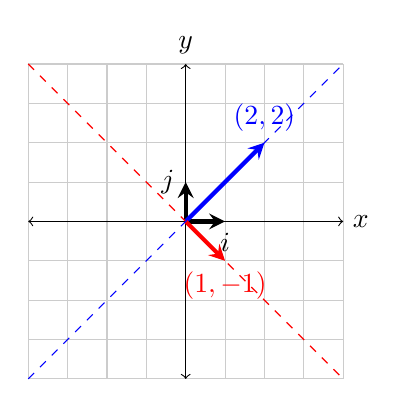
\begin{tikzpicture}[scale=0.5]
      \draw[thin,gray!40] (-4,-4) grid (4,4);
      \draw[<->] (-4,0)--(4,0) node[right]{$x$};
      \draw[<->] (0,-4)--(0,4) node[above]{$y$};
      \draw[line width=1.5pt,-stealth](0,0)--(1,0) node[anchor=north]{$i$};
      \draw[line width=1.5pt,-stealth](0,0)--(0,1) node[anchor=east]{$j$};
      \draw[line width=1.5pt,blue,-stealth](0,0)--(2,2) node[anchor=south]{$(2,2)$};
      \draw[line width=1.5pt,red,-stealth](0,0)--(1,-1) node[anchor=north]{$(1,-1)$};
      \draw[red,dashed](-4,4)--(4,-4);
      \draw[blue,dashed](-4,-4)--(4,4);
    \end{tikzpicture}
    \longrightarrow^{F}
    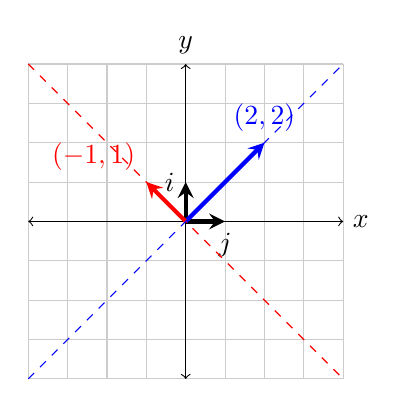
\begin{tikzpicture}[scale=0.5]
      \draw[thin,gray!40] (-4,-4) grid (4,4);
      \draw[<->] (-4,0)--(4,0) node[right]{$x$};
      \draw[<->] (0,-4)--(0,4) node[above]{$y$};
      \draw[line width=1.5pt,-stealth](0,0)--(1,0) node[anchor=north]{$j$};
      \draw[line width=1.5pt,-stealth](0,0)--(0,1) node[anchor=east]{$i$};
      \draw[line width=1.5pt,blue,-stealth](0,0)--(2,2) node[anchor=south]{$(2,2)$};
      \draw[line width=1.5pt,red,-stealth](0,0)--(-1,1) node[anchor=south east]{$(-1,1)$};
      \draw[red,dashed](-4,4)--(4,-4);
      \draw[blue,dashed](-4,-4)--(4,4);
    \end{tikzpicture}
  \end{align*}

}

\thm{}{
  Sia $ F:\mathbb{R}^n\to\mathbb{R}^n $ una applicazione lineare. F e' diagonalizzabile $ \iff $ esiste una base di $ \mathbb{R}^n $ costituita da autovettori di $ F $.
}
\pf{}{
  Dimostriamo entrambe i versi:
  \begin{itemize}
  \item Supponiamo che $ B = \{v_1,...,v_n\} $ sia una base di autovettori, e mostriamo che $ A_{BB} $ e' diagonale. Dato che sono autovettori, $ F(v) = \lambda v $, dove $ \lambda $ sono gli autovalori. Costuiamo $ A_{BB} $:
  \[
  \begin{pmatrix}
    (\lambda_1v_1)_B & ... & (\lambda_nv_n)_B\\
   \vdots & & \vdots\\
  \end{pmatrix}
  \]
  Le coordinate di $ \lambda_iv_i $ rispetto a $ B $ saranno $ (0_1, ..., \lambda_i, ..., 0_n) $, quindi forma una matrice diagonale dove i valori sulla diagonale sono gli autovalori:
      \[
        \begin{pmatrix}
  \lambda_1 & 0 & ... & 0\\
  0 & \lambda_2 & ... & 0\\
  \vdots &  &  & \\
  0 & 0 & ... & \lambda_n\\
  \end{pmatrix}
      \]
    \item Sia $ F $ diagonalizzabile. Sappiamo che esiste una base $ B $ tale che $ A_{BB} $ e' diagonale:
      \[
      A_{BB} =  \begin{pmatrix}
  \lambda_1 & 0 & ... & 0\\
  0 & \lambda_2 & ... & 0\\
  \vdots &  &  & \\
  0 & 0 & ... & \lambda_n\\
  \end{pmatrix}
      \]
      Calcolando l'immagine della base $ B $ di $ F $, abbiamo che $ \forall i \in [1,n]. F(v_i) = A_B(v_i)_B = \lambda_iv_i $, quindi $ \forall i \in [1,n].\lambda_i $ e' un autovalore di $ F $, e la base $ B $ e' formata solo da autovettori.
  \end{itemize}
}
\mprop{}{
  $ A_B $ e' diagonale $ \iff $ $ B $ e' base di autovettori
}
\pf{}{
  Dimostro entrambe i versi:
  \begin{itemize}
    \item Sia $ A_B $ diagonale e $ B = \{v_1,...,v_n\} $, seguendo lo stesso ragionamento dell'ultima dimostrazione verso la fine, abbiamo che $ \forall i \in [1,n].A_B(v_i)_B = \lambda_iv_i $, quindi tutti i vettori di $ B $ sono autovettori.
    \item Sia $ B $ una base di autovettori $ \{v_1,...,v_n\} $, dimostriamo che $ A_B $ e' diagonale. Dato che $ v_1,...,v_n $ sono autovettori, sappiamo che $ A_B(v_i)_B = \lambda_i(v_i)_B $, ovvero:
      \[
      A_B \cdot \begin{pmatrix}
      0\\
      \vdots\\
      1_i\\
      \vdots\\
      0\\
      \end{pmatrix} = \begin{pmatrix}
      0\\
      \vdots\\
      \lambda_i\\
      \vdots\\
      0\\
      \end{pmatrix}
      \]
    Quindi $ \forall i \in [1,n]. x_{1i},...,x_{i-1i} \cup x_{i+1 i},...,x_{ni} = 0 \land x_{ii} = \lambda_i $, che crea una matrice diagonale.
  \end{itemize}
}
\section{Calcolo degli autovalori e autovettori}
La definizione degli autovettori ci dice che data la matrice $ A $ associata all'applicazione lineare, $ \lambda v = Av $. Possiamo usare questa equazione per riuscire a trovare gli autovalori e di conseguenza gli autovettori, vediamo come. Trasformiamo il prodotto scalare $ \lambda v $ in un prodotto di matrici usando la matrice identita', quindi abbiamo $ (\lambda I)v = Av $. Ora portiamo tutto a destra e raccogliamo v, viene:
\[
  (A-\lambda I)v = 0
\]
Quindi stiamo cercando i vettori non nulli la cui immagine rispetto alla app. lin. $ F $ associata alla matrice $ A-\lambda I $ e' $ 0 $, ovvero il $ kerF \setminus \underline{0} $. Ma noi sappiamo che questo insieme ha elementi sse $ det(A-\lambda I) = 0 $, quindi dobbiamo trovare i $ \lambda $ che soddisfano tale richiesta. Svolgendo il determinante, otteniamo un polinomio in funzione di $ \lambda $ (il polinomio caratteristico), i cui zeri sono tutti gli autovalori di $ F $. Una volta ottenuti gli autovalori basta calcolare il nucleo delle matrici ottenute mettendo al posto di $ \lambda $ gli autovalori (l'autospazio di $ \lambda_i $), togliendo il vettore nullo.
\dfn{Polinomio caratteristico}{
  Data una matrice quadrata $ A $ definiamo \textbf{polinomio caratteristico} $ p_A $ di $ A $ il seguente polinomio in $ x $:
  \[
    p_A(x) = det(A - xI)
  \]
}
\dfn{Autospazio}{
  Dato un autovalore $ \lambda $ di una app. lin. $ F:\mathbb{R}^n\to\mathbb{R}^n $, si dice \textbf{autospazio} di $ \lambda $ il sottospazio vettoriale definito:
  \[
    V_\lambda = \{v \in \mathbb{R}^n | F(v) = \lambda v\}
  \]
}



\mprop{}{
  Sia $ T: \mathbb{R}^n\to\mathbb{R}^n $ lin. e $ v_1,...,v_k $ autovettori di $ T $, con autovalori distinti $ \lambda_1,...,\lambda_k $. Allora:
  \[
  v_1,...,v_k \text{ sono linearmente indipendenti}
  \]
}
\cor{}{
  Se $ T\colon\mathbb{R}^n\to\mathbb{R}^n $ lin. ha $ n $ autovalori distinti, allora:
  \[
  T \text{ e' diagonalizzabile}
  \]
}
\pf{}{
  Siano $ \lambda_1,...,\lambda_n $ gli autovalori di $ T $ distinti. Sappiamo quindi che $ v_1,...,v_n $ sono i rispettivi autovettori per ogni autospazio. Per la prop. sappiamo che $ v_1,...,v_n $ sono linearmente indipendenti. Quindi per GEL formano una base (fatta da autovettori), quindi $ T $ e' diagonalizzabile
}
\subsection{Molteplicita' algebrica e geometrica}
Vediamo cosa succede se ci sono degli autovalori coincidenti:
\dfn{}{
  $ A\in M_n(\mathbb{R}) $ e sia $ \lambda $ autovalore. La \textbf{molteplicita' algebrica} di $ \lambda $, indicata con $ m_a(\lambda) $ e' la massima potenza di $ (x-\lambda) $ che divide $ P_A(x) $.
}
Es: $ P_A(x) = (x-3)^5(x+2)^3(x-1)(x^2+7) $, gli autovalori sono $ \lambda_1 = 3, \lambda_2 = -2, \lambda_3 = 1 $, quindi per ognuno dobbiamo controllare il grado del fattore $ (x - \lambda) $ nel polinomio caratteristico.
\dfn{}{
    $ A\in M_n(\mathbb{R}) $ e sia $ \lambda $ autovalore. La \textbf{molteplicita' geometrica} di $ \lambda $, indicata con $ m_g(\lambda) $ e' la dimensione dell'autospazio generato da $ \lambda $.
}
\mprop{}{
  Sia $ \lambda $ un autovalore di $ A $, allora
  \[
    1 \leq m_g(\lambda) \leq m_a(\lambda)
  \]
}
\mprop{}{
  Sia $ A $ una matrice quadrata di ordine $ n $ e siano $ \lambda_1,...,\lambda_k $ i suoi autovalori distinti con molteplicita' geometriche rispettive $ n_1,...,n_k $. Sia ha che:
  \[
  n_1+...+n_k = n \iff A \text{ e' diagonalizzabile}
  \]
}
\mprop{}{
  $ F:\mathbb{R}^n\to\mathbb{R}^n $ e' diagonaliz $ \iff $ esiste una base di $ \mathbb{R}^n $ costituita di autovettori. Gli autovalori sono le radici del polinomio caratteristico $ p_A(x) $ con $ F = L_A $ che ha grado $ n $. 
}
Fattorizziamo $ p_A(x) $ e troviamo i suoi zeri. $ m_a(\lambda) $ ci dice quante volte compare uno zero, ma a noi interessa la dimensione dell'autospazio $ m_g(\lambda) $ perche' ci servono gli autovettori.
\mprop{}{
  \[
    1 \leq m_g(\lambda) \leq m_a(\lambda)
  \]
}
Per avere una base di autovettori, se $ \lambda_1, ..., \lambda_k $ sono gli autovalori, deve essere $ dimV_{\lambda_1} + ... + dimV_{\lambda_k} $. Deve valere che $ m_a(\lambda_1) + ... + m_a(\lambda_k) = n $ e $ m_a(\lambda_i) = m_g(\lambda_i) $. La prima condizione vuol dire che $ p_A(x) $ si fattorizza completamente, ovvero che ha $ n $ zeri, la seconda ci dice che la dimensione dell'autospazio deve essere quello "massimo".
\mprop{}{
  sia $ F\colon\mathbb{R}^n\to\mathbb{R}^n $, con autovalore $ 0 $, $ \exists v \in \mathbb{R}^n.v\neq \underline{0} \land F(v) = 0v = \underline{0} \implies v \in kerF $
}
Quindi $ V_0 = kerF \neq \{0\} \implies F $ non e' iniett $ \implies F $ non e' invertibile
\nt{
  diagonaliizzabile $ \nRightarrow $ invertibile e viceversa
}
\mprop{}{
  Matrici simili hanno lo stesso polinomio caratteristico (non vale l'opposto)
}
\nt{
  Quindi cambiando le basi ad una matrice, il polinomio non cambia (purche' siano le stesse al dominio e codominio)
}
\chapter{Prodotto Scalare Euclideo}
Sul libro si chiama 'prodotto scalare definito positivo', ma non lo seguiamo esattamente.\\
Siano $ v=(v_1,v_2), w=(w_1,w_2) $, il prodotto scalare si indica con $ <v,w> $ (non e' il sottospazio!) ed e' un numero. Osserviamo che $ <v,w> = |v||w|cos\theta $, dove $ \theta $ e' l'angolo convesso formato dalle semirette di $ v $ e $ w $.
\mprop{}{
  Il prodotto scalare fra due vettori del piano $ v=(x_1,y_1), w=(x_2,y_2) $, allora un'altra formula per ottenere il loro prodotto scalare e':
  \[
  <v,w> = x_1x_2+y_1y_2
  \]
  Si puo' espandere in $ \mathbb{R}^n $
}
In altre parole si puo' vedere il prodotto scalare fra due vettori come il prodotto di due matrici (una a riga e l'altra a colonna):
\[
  <v,w> = v\cdot w^T = (v_1,...,v_n)\cdot \begin{pmatrix}
  w_1\\
  \vdots\\
  w_n\\
  \end{pmatrix} = v_1w_1+...+v_nw_n
\]
\section{Proprieta'}
Possiamo quindi vedere il prodotto scalare come una funzione che prende due vettori di $ \mathbb{R}^n $ e ci restituisce uno scalare: $ <\cdot,\cdot>: \mathbb{R}^n \times \mathbb{R}^n \to \mathbb{R} $, che gode di varie proprieta':
\begin{itemize}
\item \textbf{Simmetria}: $ \forall x,y \in \mathbb{R}^n. <x,y> = <y,x> $
\item $ \forall x,y,z \in \mathbb{R}^n. <x+z, y> = <x,y>+<z,y> $
\item $ \forall x,y \in \mathbb{R}^n, \lambda \in \mathbb{R}. <\lambda x, y> = \lambda <x,y> $
\end{itemize}
Notiamo che se fissiamo $ y $, questa funzione diventa lineare. Inoltre, grazie alla simmetria, possiamo applicare le prop. 2 e 3 anche a $ y $. Quindi fissando $ x $ otteniamo nuovamente una funzione lineare, per questo motivo il prodotto scalare e' detto \textbf{bilineare}.
\begin{itemize}
\item $ \forall x \in \mathbb{R}^n. <x,x> \geq 0 \land <x,x> = 0 \iff x = \underline{0} $
\end{itemize}
Questa ultima proprieta' ci dice che il prodotto scalare ha forma \textbf{definita positiva} e ci consente di dare la seguente definizione:
\dfn{Norma}{
  Dato un vettore $ v = (v_1,...,v_n) \in \mathbb{R}^n $, si dice \textbf{norma} di $ v $ la "lunghezza" del vettore che parte dall'origine $ (0,...,0) $ e arriva a $ (v_1,...,v_n) $ e si calcola in tale modo:
  \[
  ||v|| = \sqrt{<v,v>} = \sqrt{v_1^2+...+v_n^2}
  \]
}
\section{Ortogonalita'}
\dfn{Vettori ortogonali}{
  Due vettori $ v,w \in \mathbb{R}^n $ si dicono \textbf{ortogonali} se l'angolo compreso fra di loro e' $ \frac{\pi}{2} $, ovvero quando:
  \[
  <v,w> = 0
  \]
}
Seguendo questa definizione, l'ortogonalita' gode delle seguenti proprieta':
\begin{itemize}
  \item $ \forall x,y \in \mathbb{R}^n. x \perp y \iff y \perp x $ (simmetria)
  \item $ \forall x,y,z \in \mathbb{R}^n. x \perp y \land x \perp z \iff x \perp \lambda y + \mu z $
\end{itemize}
Quest'ultima proprieta' ci dice che se un vettore e' ortogonale rispetto ad altri due vettori, allora e' ortogonale rispetto a tutti i vettori appartenenti al sottospazio vettoriale formato dai due vettori. Allora possiamo dire che:
\mprop{Indipendenza lineare di vettori ortogonali}{
  Presi dei vettori non nulli $ v_1,...,v_k \in \mathbb{R}^n $ ortogonali fra di loro, questi sono \textit{linearmente indipendenti}
}
\pf{}{
  Dati $ k $ vettori non nulli $ v_1,...,v_k $ ortogonali, dimostriamo che $ \lambda_1v_1+...+\lambda_kv_k = \underline{0} \implies \lambda_1,...,\lambda_k = 0 $. Sappiamo che $ \forall i = 1,...,j $, $ <\lambda_1v_1+...+\lambda_kv_k, v_i> = 0 $, dato che il prodotto scalare per il vettore nullo e' sempre zero. Usando la bilinearita', possiamo trasformare il prodotto scalare $ \lambda_1<v_1,v_i>+...+\lambda_i<v_i,v_i>+...+\lambda_k<v_k,v_i> = 0 $, togliendo i prodotti scalari che per ortogonalita' sono nulli, ci rimane (usando la definizione di norma) $ \lambda_i||v_i||^2 = 0 $. Dato che $ v_i $ non e' nullo per ipotesi, abbiamo che $ \forall i = 1,...,k. \lambda_i = 0 $.  
}

\dfn{Base ortonormale}{

  I vettori $ v_1,...,v_n $ si dicono \textbf{ortonormali} se $ <v_i,v_j> = \begin{cases}
  1 & i = j\\
  0 & i\neq j
  \end{cases} $. Cioe' se sono tutti lunghi $ 1 $ e perpendicolari
}
Le basi ortonormali hanno la caratteristica per cui facendo il prodotto scalare di un vettore con ognuno dei vettori della base si ottiene la coordinata (rispetto alla base) corrispondente, ovvero:
\mprop{}{
  Data una base ortonormale $ B = \{v_1,...,v_n\} $ e un vettore $ v $ con coordinate rispetto a $ B $ $ (\lambda_1,...,\lambda_k) $, si ha che:
  \[
  \forall i = 1,...,n. <v,v_i> = \lambda_i
  \]
}
Cio' coincide con l'interpretazione geometrica del prodotto scalare, in quanto i $ \lambda $ trovati in questo modo corrispondono al modulo del vettore proiettato su ciascun vettore della base.

\section{Sottospazi ortogonali}
\dfn{Sottospazio ortogonale}{
  Dato uno sottospazio $ W \leq \mathbb{R}^n $, si chiama \textbf{sottospazio ortogonale} di $ W $ l'insieme degli elementi di $ \mathbb{R}^n $ che sono ortogonali a tutti i vettori di $ W $, ovvero:
  \[
  W^\perp = \{v \in \mathbb{R}^n | \forall w \in W. <v,w> = 0\}
  \]
}
\mprop{}{
  Tutti i sottospazi ortogonali sono sottospazi vettoriali
}
\mprop{}{
  Dato un sottospazio $ W $ con base $ v_1,...,v_k $, il suo sottospazio ortogonale e' formato da:
  \[
  W^\perp = \{v \in \mathbb{R}^n | \forall i = 1,...,k. <v,v_i> = 0 \}
  \]
  Ovvero, per vedere se un vettore e' ortogonale a tutti i vettori di un sottospazio, basta controllare che sia ortogonale ai vettori base.
}
\pf{}{
  Si dimostra usando la dipendenza lineare e la bilinearita' del prodotto scalare.
}
\subsection{Algoritmo di Gram-Schmidt}
Grazie a questa proposizione, abbiamo un modo per trovare la base del sottospazio ortogonale data la base di qualunque sottospazio. Vediamo un algoritmo per ottenere proprio questo:
(algoritmo di gram)


\mprop{Dimensione sottospazio ortogonale}{
  Dato un sottospazio $ W $ di $ \mathbb{R}^n $, allora:
  \[
  dimW^\perp = n - dimW
  \]
  Inoltre, $ W \cap W^\perp = \{\underline{0}\} $
}
\chapter{Aritmetica modulare}


\end{document}

